\documentclass[a4paper]{article} 	% use "amsart" instead of "article" for AMSLaTeX format

\usepackage{geometry}  		% See geometry.pdf to learn the layout options. There are lots.
\geometry{left=1.5cm,right=1.5cm,top=1.5cm,bottom=1.5cm}   		
\usepackage{graphicx,subcaption}					
\usepackage{amssymb}
\usepackage{indentfirst}
\usepackage{amsmath}
\usepackage{amsthm}
\usepackage{bm}
\usepackage{lineno}
\usepackage{setspace}
\usepackage{booktabs,multirow}
\usepackage{authblk}
%\usepackage{subcaption}
\usepackage{float}
\usepackage[flushleft]{threeparttable} % For adding footnotes to tables


\RequirePackage[colorlinks,citecolor=blue,urlcolor=blue]{hyperref}

\newtheorem{theorem}{Theorem}
\newtheorem{lemma}[theorem]{Lemma}
\newtheorem{corollary}[theorem]{Corollary}
\newcommand{\E}{\mathrm{E}}
\newcommand{\D}{\mathcal{MD}}
\newcommand{\Var}{\mathrm{Var}}
\newcommand{\Cov}{\mathrm{Cov}}
\newcommand{\Corr}{\mathrm{Corr}}
\newcommand{\tr}{\mathrm{tr}}
\newcommand{\R}{\texttt{R}}
\newcommand{\asreml}{\texttt{ASReml-R}}
\newcommand{\Matern}{Mat\'ern }
\newcommand{\N}{\mathcal{N}}
\newcommand{\AR}{\mathrm{AR1}}
\newcommand{\BigO}[1]{{\rm O}\left(#1\right)}
\newcommand{\eg}{e.g.\ }
\newcommand{\ie}{i.e.\ }
\newcommand{\iid}{\textrm{i.i.d.\ }}

\newcommand{\revision}[1]{\textcolor{red}{#1}}


\usepackage[url=false, isbn=false, eprint=false, backref=true, style= authoryear, backend=biber, maxcitenames=2, giveninits=true, maxbibnames=100, uniquename=init]{biblatex}   %% backend=bibtex
\DeclareNameAlias{sortname}{family-given}
\addbibresource{REF.bib}

\title{\textbf{The Diary of an Ordinary Man}}
\author{Tongji University Automotive Institute :\textbf{2351071 Zhang hengzhen}}
%\author[1]{First Author Name %\thanks{Corresponding author: email@example.com}}
%\author[1,2]{Second Author}
%\author[2]{Third Author}



%\affil[1]{Affiliation one}
%\affil[2]{Affiliation two}
 
\date{}							
% Activate to display a given date or no date

%\linenumbers
\doublespacing
%\onehalfspacing

\begin{document}

\maketitle

As the semester draws to a close, it's time to reflect on the academic journey that has shaped both my intellectual and personal growth. This collection of weekly diaries is more than just a record of events—it's a narrative of my thoughts, challenges, and progress over the past several months. Each diary represents a snapshot of my experiences, from grappling with complex concepts to celebrating small victories in learning.

Through the act of writing these reflections, I have learned to articulate my ideas more clearly and thoughtfully, while also gaining a deeper appreciation for the learning process itself. This final diary serves as a conclusion to this chapter of my academic life, offering both closure and a glimpse into the future challenges that await.
\section{Week 1 Diary: A Fresh Start}

As I embark on this new semester, I can’t help but feel the weight of my aspirations pressing down on me like a heavy textbook. This term, more than any before, is a crucial stepping stone toward achieving the goals I’ve set for myself: excelling academically, participating in high-quality competitions, and, if the stars align, securing a spot in my professor’s research group. 

The pressure to improve my GPA is palpable, especially with the new grading standards in place for each of my courses. From advanced calculus to academic English writing, the complex breakdown of points for attendance, projects, and exams means that every single task could affect my final score. Take, for example, **Material Mechanics** with its careful weighting—0.1 for attendance, 0.1 for homework, 0.2 for the midterm, and a daunting 0.6 for the final exam. And let’s not forget **Statistical Probability**, where two tests and a final exam account for the majority of the grade, meaning no moment of rest. Every lesson, every problem set, is a potential turning point.

\subsection*{The Path to Excellence}

But beyond the desire to simply keep my GPA afloat lies a deeper ambition. I want to go beyond coursework—to challenge myself with real-world problems and innovative solutions. I’ve set my sights on participating in engineering practice competitions, as well as high-level mathematical modeling contests. These aren’t just extracurricular activities; they are essential stepping stones that could open the doors to research opportunities and prestigious positions within my professor’s projects.

I know this won’t be easy. The competition will be fierce, and the bar is set high. But that only adds to the excitement. The prospect of applying what I’ve learned—whether it’s using linear programming to solve agricultural planning problems or mastering mechanical principles for innovative designs—fills me with a sense of purpose. Each formula, each algorithm, brings me closer to the edge of discovery.

\subsection*{Grading Standards and the Fight for a Higher GPA}

Of course, none of this is possible without mastering the coursework first. The grading standards this semester are especially rigorous. For example, **Academic English Writing** is broken down into multiple components: attendance (0.1), class performance (0.3), and two projects (0.2). To top it off, the final is split between a paper and a presentation, leaving no room for error.

For each class, the final exam looms like a mountain in the distance, its shadow growing larger as the weeks go by. It’s not just about passing—it’s about excelling. And with each class requiring a different strategy, it feels like I’m playing a complex game of chess, where every move could determine the outcome of my GPA.

\begin{figure}[h!]
	\centering
	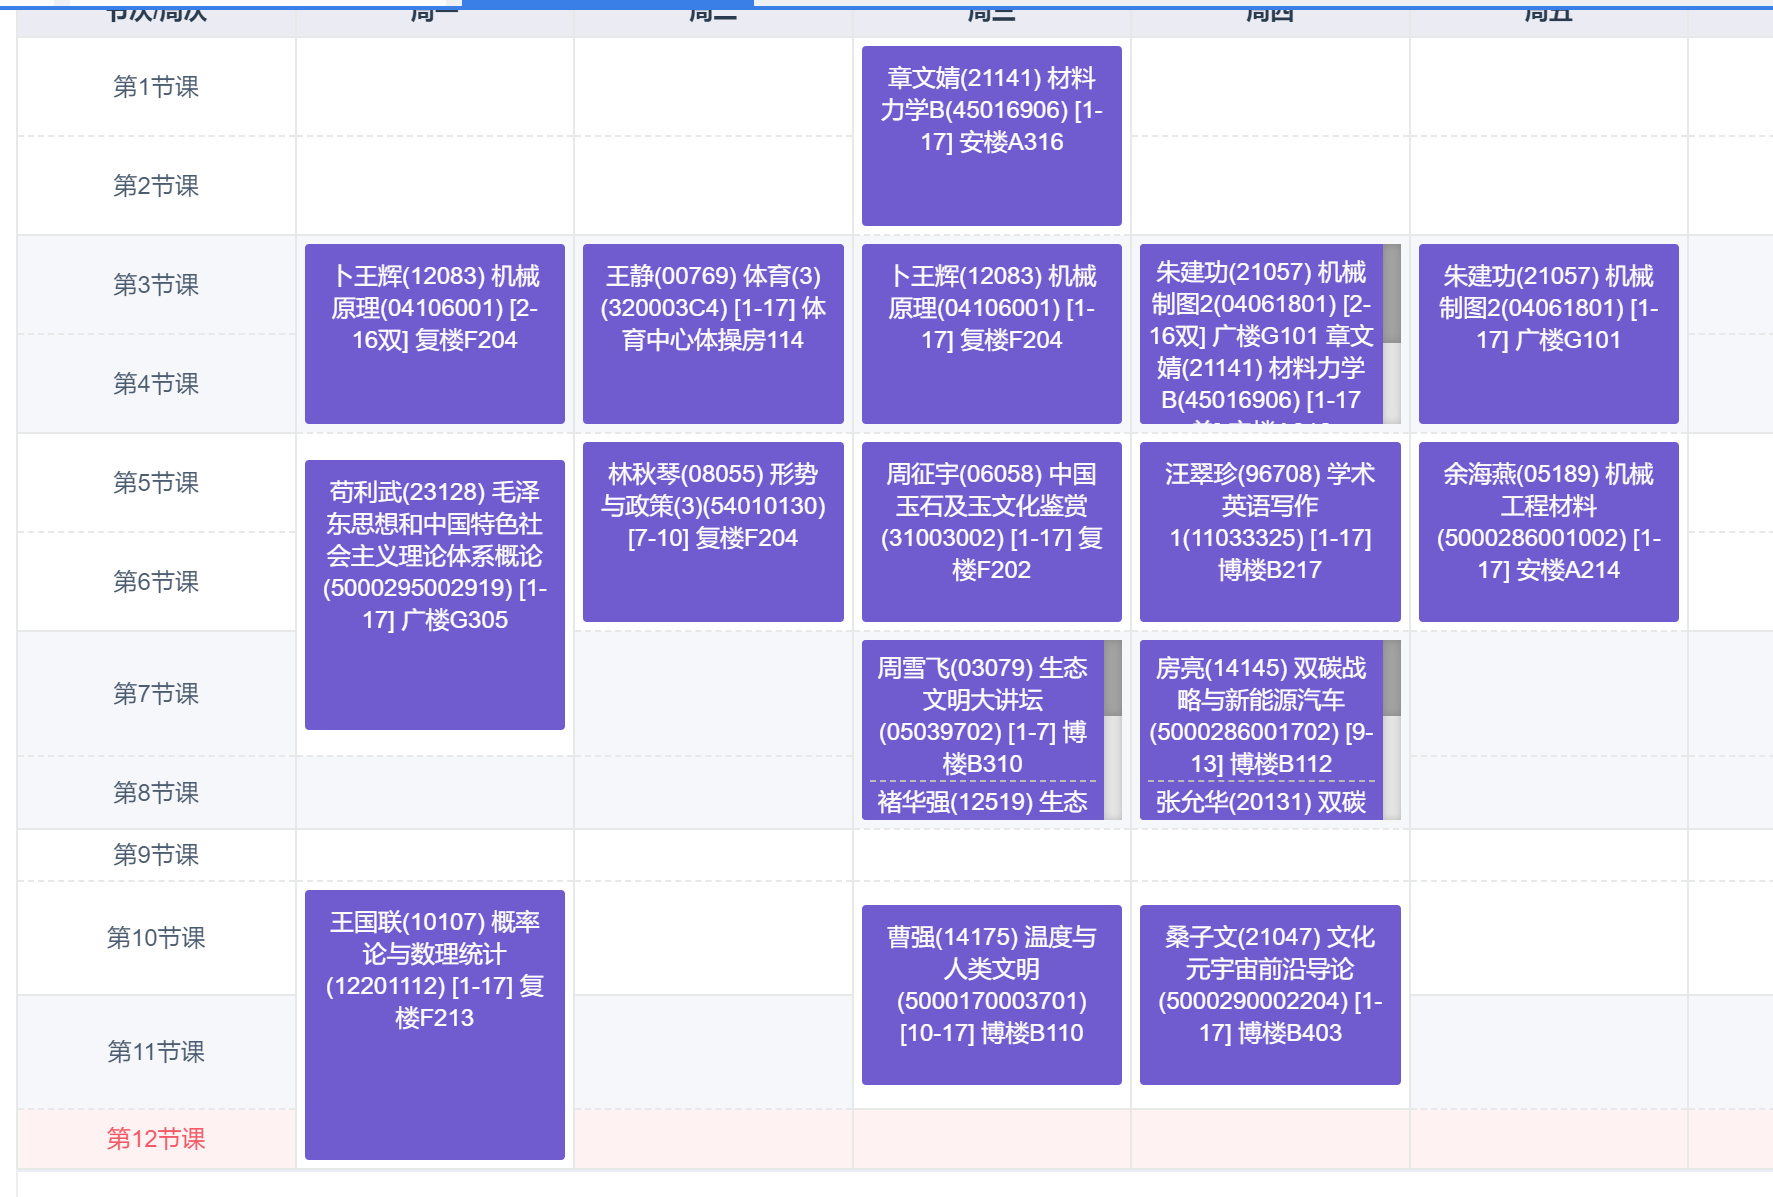
\includegraphics[width=0.8\textwidth]{fig001.png}  % Replace "example-image" with the file name of your image
	\caption{timetable}
	\label{fig:001}
\end{figure}

\subsection*{The Drive to Succeed}

This semester, I am more determined than ever. The goals I’ve set for myself are ambitious, but they are also the key to unlocking future opportunities. Whether it’s entering the **Advanced Mathematics Competition**, securing a spot in an engineering contest, or finally getting a chance to work with my professor, I know that the work I put in now will pay off in the long run.

And so, I take on this semester with a mixture of excitement and nervous anticipation. I know it will be challenging, but the rewards are worth the effort. My GPA, my academic achievements, and my future success all depend on how well I navigate these next few months. Here's hoping that, with hard work and a little bit of luck, I’ll come out on top.

\section{Week 2 Diary: Participating in the Mathematical Modeling Competition}

This week was an unforgettable journey into the world of mathematical modeling. I found myself fully immersed in the challenge of solving real-world agricultural problems using orthogonal experimental design and linear programming. The task? To optimize crop planting strategies for rural farmers. The reality? Far more challenging than anticipated. 

Theoretically, the solution seemed straightforward: define the constraints, set up the objective function, and let MATLAB do the heavy lifting. Oh, how naive I was! The journey from theory to implementation felt like traversing a battlefield, where the main enemies were syntax errors, memory overflows, and MATLAB crashes.

\subsection*{Orthogonal Experiment Design and Linear Programming in Action}

We applied orthogonal experimental design to identify the key factors influencing agricultural profit margins. This method helped streamline the number of experiments needed while maximizing the reliability of the results. Following this, we employed linear programming to create a model that balanced profit expectations with worst-case scenario protection. The result was a robust planting strategy that could theoretically increase total profit by nearly 20\%. A practical contribution to solving real-world agricultural issues, no doubt.

\begin{figure}[h!]
	\centering
	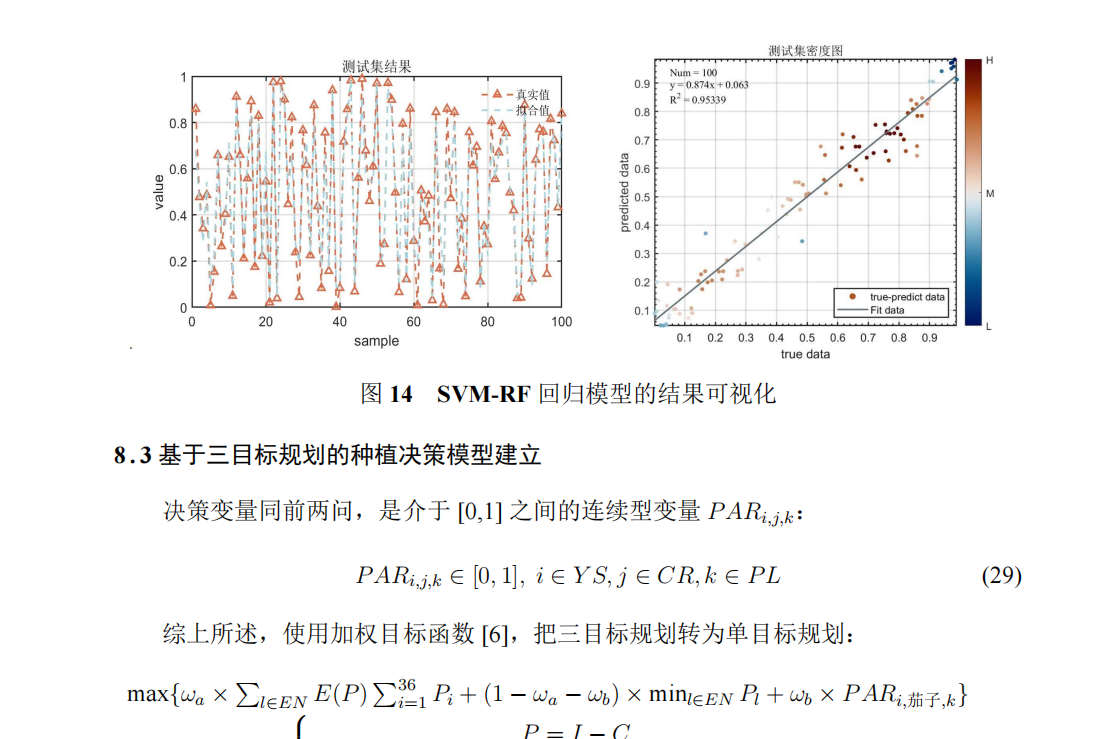
\includegraphics[width=0.8\textwidth]{fig002.png}  % Replace "example-image" with the file name of your image
	\caption{Orthogonal Experiment Design and Linear Programming in Action}
	\label{fig:002}
\end{figure}

However, as elegant as the mathematical models were, the implementation was far from it. MATLAB, my trusted companion, became the most temperamental partner. At some point, I lost count of how many times I had to restart after a crash. The code—oh, the code—was a constant battle of debugging, rewriting, and optimizing. You know the struggle is real when your computer’s beeping alarm haunts your dreams. 

\subsection*{The Code and the Beeping Computer}

Imagine sitting in front of a screen, lines of code blurring into one another. Then, like a siren’s song, you hear the cold, mechanical voice of your computer's warning: \textit{TypeError: 'int' object is not subscriptable}. These aren’t just error messages—they are the lullabies of frustration, whispering the cold reality that your code is, yet again, broken.

But once you’ve been pulled into the labyrinth of debugging, like a spider's prey caught in its web, there is no turning back. Some things, once begun, cannot be left unfinished. Sleep? A distant memory. Over three days, I accumulated a grand total of nine hours of sleep. My nights were spent in the dim glow of my screen, coaxing MATLAB into submission while praying that the next run wouldn't end in another crash. 

\subsection*{Three Days, Nine Hours of Sleep, and a Completed Paper}

After three days of constant coding, troubleshooting, and rewriting, I finally finished the paper. The feeling of relief was indescribable. I had poured my heart and soul into it, along with several sleepless nights. Whether it was the orthogonal experiments, linear programming, or just the sheer amount of caffeine consumed, I managed to complete everything on time. Now, I can only hope for a good result. 

Looking back, this competition taught me not only about advanced mathematical techniques but also about perseverance and endurance. Sure, I may have lost some sleep, but the satisfaction of solving complex problems and applying mathematical models to real-world scenarios made it all worthwhile. Now, I wait in hopeful anticipation of the results, wishing for a well-deserved victory. 

\subsection*{Conclusion}

In conclusion, this week was an intense but rewarding experience. Despite the challenges—mainly a rebellious MATLAB and the relentless beeping of my computer—I managed to contribute a practical solution to the agricultural problem. Whether or not I get a good result in the competition, I feel proud of the work I’ve done. After all, as they say, "the journey is the reward."

\section{Week 3 Diary: Creating a Metaverse Grid Game Demo}

This week was nothing short of an adventure in both programming and the metaverse! For my elective course, *Frontier Introduction to Cultural Metaverse*, I had to prepare both a presentation and a paper. As an ambitious student with limited experience in game development, I decided to push my boundaries by creating a small demo for a metaverse-inspired grid game using Python, HTML, CSS, and JavaScript.

It turns out, diving headfirst into technologies I had never used before wasn’t as daunting as I feared—thanks to some good old-fashioned help from generative AI. My chosen AI companion for this challenge? GPT-4o. I went from having zero experience in Pygame or web development to releasing a functional game demo in just two hours. Talk about a technological miracle!

\subsection*{The Process of Game Development: Aided by GPT-4o}

Let me take a moment to paint a picture of my workflow. Armed with the basic idea for a grid-based game, I approached GPT-4o to assist me in crafting the code. From walking me through installing Pygame to generating HTML code snippets, GPT-4o became my indispensable mentor. It was like having a patient, tireless tutor guiding me step by step, filling the gaps in my knowledge as I tackled unfamiliar programming concepts.

The result? A charming little grid game demo that my classmates and roommates genuinely enjoyed. With simple controls, the player moves through a metaverse-like environment, experiencing the thrill of exploration in a minimalist world. Honestly, it was beyond my wildest expectations! I uploaded the entire project to GitHub to share it with the world, feeling both proud and slightly astonished at how quickly I had crossed the finish line.

Reflecting on the process, I couldn’t help but think of that news article I read recently. An 8-year-old kid, with the help of Claude3.5, managed to develop a website and create a game all on their own. The speed at which AI is democratizing programming knowledge is nothing short of breathtaking. We are living in a time where beginners like me, or even kids, can develop games in hours—without any prior experience. The learning curve has never been this shallow, and the opportunities, endless.

\begin{figure}[h!]
	\centering
	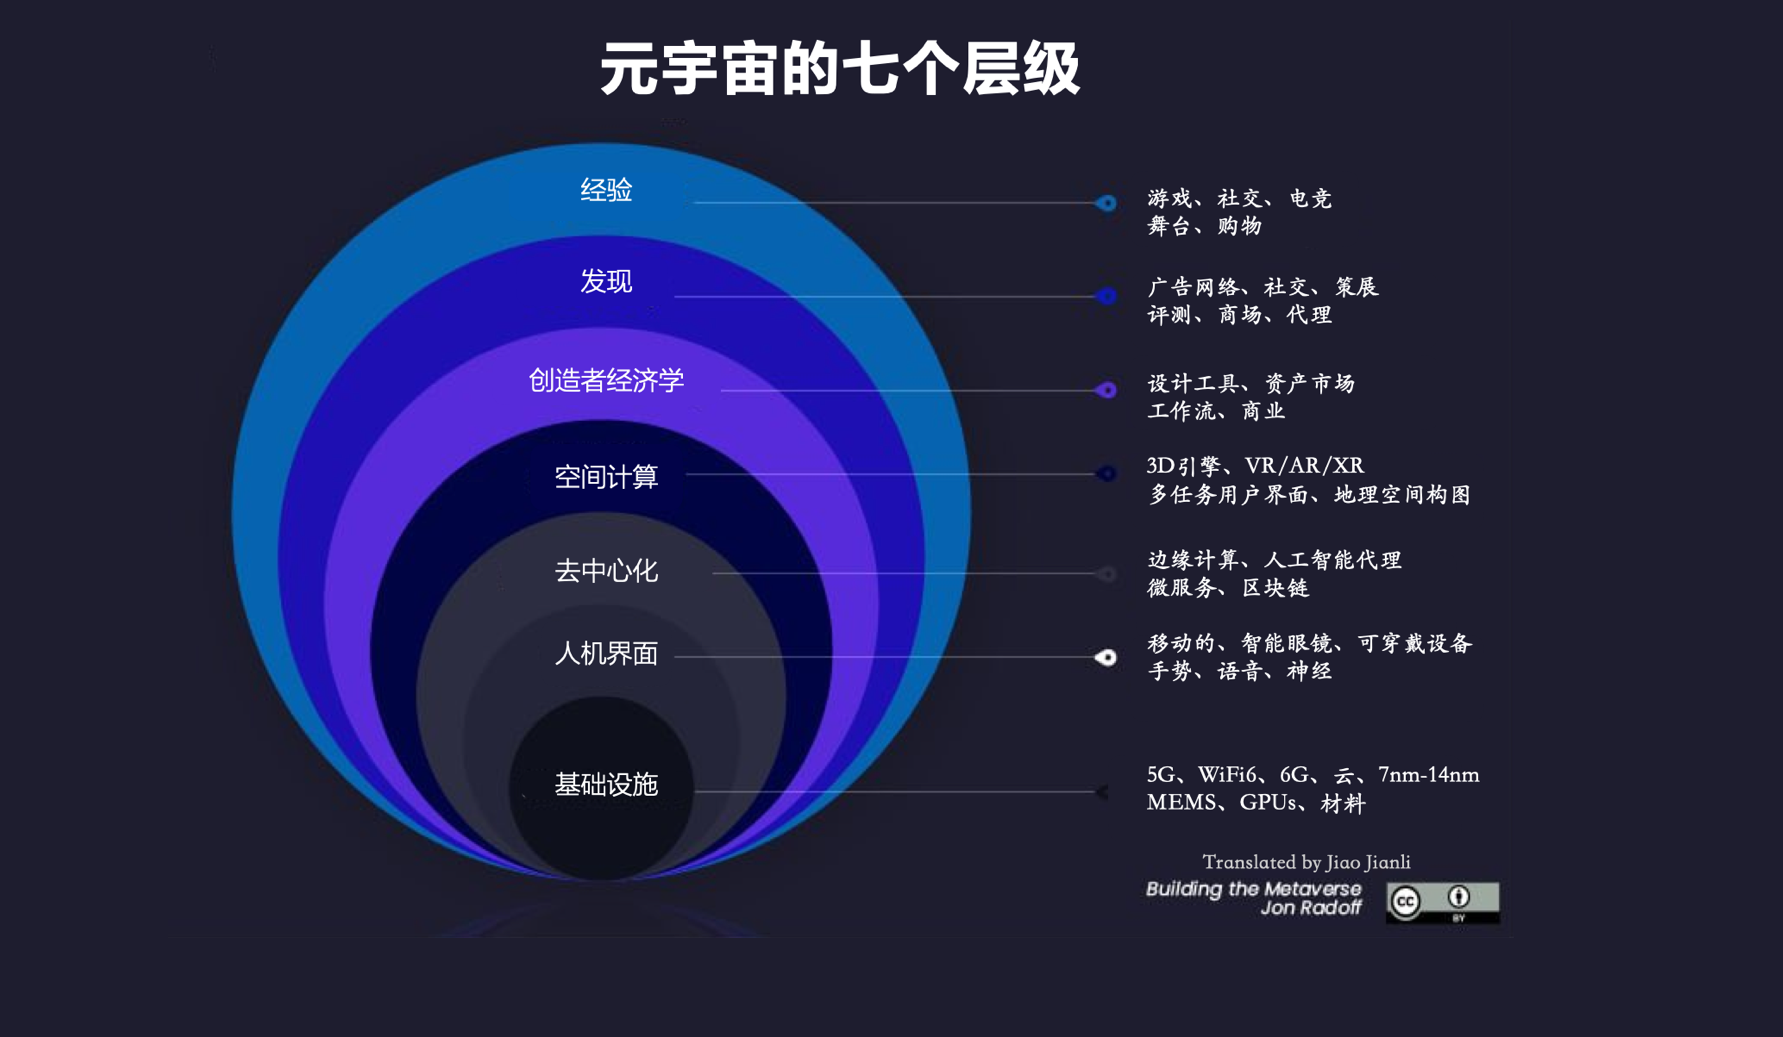
\includegraphics[width=0.6\textwidth]{fig004.png}  % Replace "example-image" with the file name of your image
	\caption{Exploring the Metaverse and Game Development}
	\label{fig:003}
\end{figure}

\subsection*{Exploring the Metaverse and Game Development}

But the technical achievements were only part of the story. This whole exercise was intertwined with the broader context of my course on the metaverse. I took this opportunity to dive deeper into the development potential of open-world exploration games within the metaverse, analyzing the business model of MiHoYo, the Chinese gaming company behind massive hits like *Genshin Impact* and *Honkai: Star Rail*.

MiHoYo’s success is rooted in its ability to combine an immersive open-world experience with gacha mechanics that fuel player engagement. The metaverse, I realized, is not just about virtual reality headsets and augmented worlds. It’s also about crafting dynamic and engaging spaces where users want to spend their time, exploring, creating, and interacting. Companies like MiHoYo have mastered this balance, offering a glimpse into what future metaverse games might look like.

\subsection*{Leveraging AI for Academic Work}

Finally, I must give credit to GPT-4o for more than just the game demo. The AI also helped me streamline my academic work. I used it to generate LaTeX code for my paper and employed Python’s `pptx` library to craft my PowerPoint slides. What used to take me days—writing a polished paper and preparing a coherent presentation—was now condensed into hours of efficient work.

Looking back, this week has been a perfect blend of academic research, technical challenges, and creative expression. From writing code with AI assistance to gaining insights into the future of metaverse gaming, I’ve had a uniquely productive and insightful experience. Now, I just hope my presentation and paper receive as much praise as my game demo!

\subsection*{Conclusion}

In conclusion, this week’s journey into game development and the metaverse was both challenging and rewarding. With the help of GPT-4o, I managed to go from a complete novice in Pygame and web development to a proud creator of a functional game demo. Along the way, I explored new frontiers in metaverse gaming and utilized AI to accelerate my academic work. It’s safe to say that this week has been a demonstration of just how fast technology—and my understanding—can evolve.

\section{Week 4 Diary: YOLOv10 Pedestrian Detection Paper Accepted}

This week was a monumental milestone in my academic journey—my paper on the real-time pedestrian detection algorithm,\textbf{ YOLOv10}, was accepted for publication at the Q\textbf{uantum-enhanced Machine Learning workshop (CDSCH 2024)}! As thrilling as this achievement is, the process behind it wasn’t without its challenges. Nevertheless, it feels incredible to see my work finally recognized, and I even uploaded the code to GitHub: \href{https://github.com/weyumm/YOLOv10-Pedestrian-Detection}{YOLOv10-Pedestrian-Detection}. 

The paper, titled “\textbf{Research on Real-time Pedestrian Detection Algorithm of YOLOv10 under Complex Lighting and Occlusion Conditions},” dives deep into the YOLOv10 architecture and explores how it can handle the often tricky conditions of lighting changes and occlusion during pedestrian detection. 

\subsection*{YOLOv10: An Algorithm for Complex Scenarios}

For those unfamiliar, YOLOv10 is a state-of-the-art deep learning model designed for object detection, specifically optimized for real-time tasks. My work focused on pushing this algorithm’s capabilities to handle difficult pedestrian detection tasks under complex lighting and occluded environments. These conditions are particularly important for applications like intelligent traffic monitoring and autonomous driving, where pedestrian safety is paramount.

The core improvements introduced in YOLOv10 include:
\begin{itemize}
	\item \textbf{Dual-label assignment system}: This ensures more accurate bounding boxes by utilizing multiple label assignments during training.
	\item \textbf{Compact inverted block (CIB)}: A novel feature that enhances the model’s ability to generalize across various scales of pedestrians.
	\item \textbf{Partial self-attention (PSA)}: This feature strengthens the model’s ability to handle occlusions by improving the global context perception.
\end{itemize}

My experiments showed that YOLOv10 achieved a \textbf{93.4\% mAP} (mean Average Precision) on the expanded Caltech pedestrian dataset, which is a significant improvement over YOLOv8. Moreover, the algorithm maintained a small number of parameters (20.4M), making it both efficient and highly accurate for real-time detection.

\begin{figure}[h!]
	\centering
	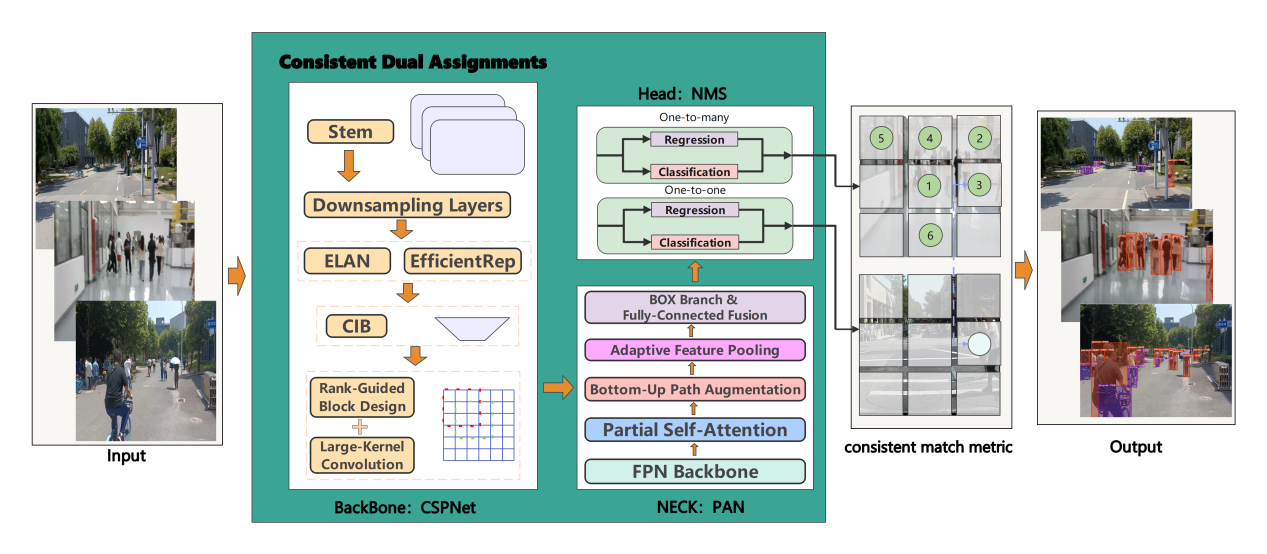
\includegraphics[width=1.0\textwidth]{fig0033.png}  % Replace "example-image" with the file name of your image
	\caption{Orthogonal Experiment Design and Linear Programming in Action}
	\label{fig:0031}
\end{figure}

\subsection*{Challenges with Code and GitHub Success}

Now, while the paper was a success, the journey to writing and testing the code was, let’s say, an adventure. My computer’s CPU fan seemed to scream in protest as I ran endless rounds of training and testing. There were multiple nights spent debugging obscure errors that seemed to come from the depths of the machine learning abyss. However, with enough perseverance—and the help of my trusty AI assistant, GPT-4o—I managed to refine the code.

I eventually pushed the full codebase to GitHub, where it gained attention from fellow researchers and students. For someone who had never fully published a project online before, this felt like a great achievement. The repository, complete with detailed documentation, is now publicly available for anyone interested in pedestrian detection. Feel free to check it out and give it a star! \url{https://github.com/weyumm/YOLOv10-Pedestrian-Detection}

\subsection*{The Power of AI Assistance and Perspective}

Looking back, I couldn’t help but recall a story I read about an 8-year-old using AI to build their first website and game. It’s both humbling and inspiring to think about how rapidly AI tools, like GPT-4o, are changing the landscape of programming and research. Here I am, using advanced models to push the boundaries of pedestrian detection, while kids are creating websites with AI assistance. It’s a clear sign that we are living in a transformative era of technology.

What this experience taught me is that the tools available today can enable anyone to accomplish incredible feats, no matter their prior experience. The future of research and development in fields like computer vision, autonomous systems, and the metaverse is incredibly bright, and I’m excited to be part of it.

\subsection*{Conclusion}

In conclusion, this week has been a whirlwind of emotions, from the excitement of my paper being accepted to the technical trials of pushing code to GitHub. YOLOv10 has shown its strength in tackling the challenges of real-time pedestrian detection under complex conditions, and I couldn’t be more proud of my contribution to this growing field. The power of AI, both in helping us solve complex problems and making tools accessible, continues to amaze me. Now, I eagerly await the conference and the chance to share my work with the broader academic community.

\section{Week 5 Diary: SITP Mid-term Report:Mathematical Textbook Translation Based on Large Model Fine-tuning.}

As part of the University Innovation and Entrepreneurship Project (SITP), this week marked a major checkpoint in our progress on “\textbf{Mathematical Textbook Translation Based on Large Model Fine-tuning.}” Our goal is ambitious: utilizing cutting-edge neural machine translation techniques to translate highly specialized mathematical content, ensuring accuracy while maintaining readability for non-native speakers.

To say that this has been a learning curve would be an understatement. As the project’s mid-term report approached, we delved deep into the history and development of machine translation, explored datasets, and navigated the intricacies of fine-tuning large language models. In this diary entry, I’ll recap our journey so far and share some thoughts on what lies ahead.

\subsection*{Evolution of Machine Translation: From Rules to AI}

As part of our research, we explored the evolution of machine translation (MT) from its humble beginnings to the present day. We learned that MT has progressed through three main stages: rule-based translation, statistical translation, and finally, neural machine translation (NMT). Each stage marked a significant improvement in both the quality and speed of translation, but NMT, powered by deep learning, is where we’ve seen truly revolutionary progress.

Our project, of course, focuses on NMT. We are leveraging a large model fine-tuning approach, which allows us to adapt pre-trained models to the specific needs of mathematical language. Given the complexity and precision required in mathematical terminology, this is no small feat, but it’s exciting to be working at the cutting edge of both machine learning and translation.

\subsection*{Dataset Management: Divide and Conquer}

The backbone of any machine learning project is the dataset, and ours is no exception. Our project involves carefully dividing the data into three parts: the \textbf{training set}, \textbf{the validation set}, and the \textbf{test set}. The training set is used to teach the model, the validation set helps fine-tune hyperparameters, and the test set provides an unbiased evaluation of the model’s performance.

In our case, we’ve been working with a dataset of bilingual (Chinese-English) pairs from mathematical textbooks, along with an English-to-Chinese dictionary of technical terms. This combination is essential for ensuring the translation remains accurate across a wide range of mathematical concepts. The dictionary also plays a critical role in improving the model’s ability to handle domain-specific terms, avoiding confusion that might arise from direct, context-agnostic translations.

\subsection*{Challenges in Mathematical Textbook Translation}

One of the biggest challenges we’ve faced so far is ensuring the translated text maintains the same level of precision as the original. Unlike general language translation, where some flexibility can be tolerated, translating mathematical textbooks requires utmost precision. Even a minor error in translating a formula or theorem could lead to misunderstandings for the reader.

Another significant challenge has been dealing with the issue of \textbf{multimodal translation}, which arises from the fact that mathematical textbooks often include both text and equations. We need to ensure that the model can handle and appropriately translate both forms of content, without distorting meaning or introducing errors.

\begin{figure}[h!]
	\centering
	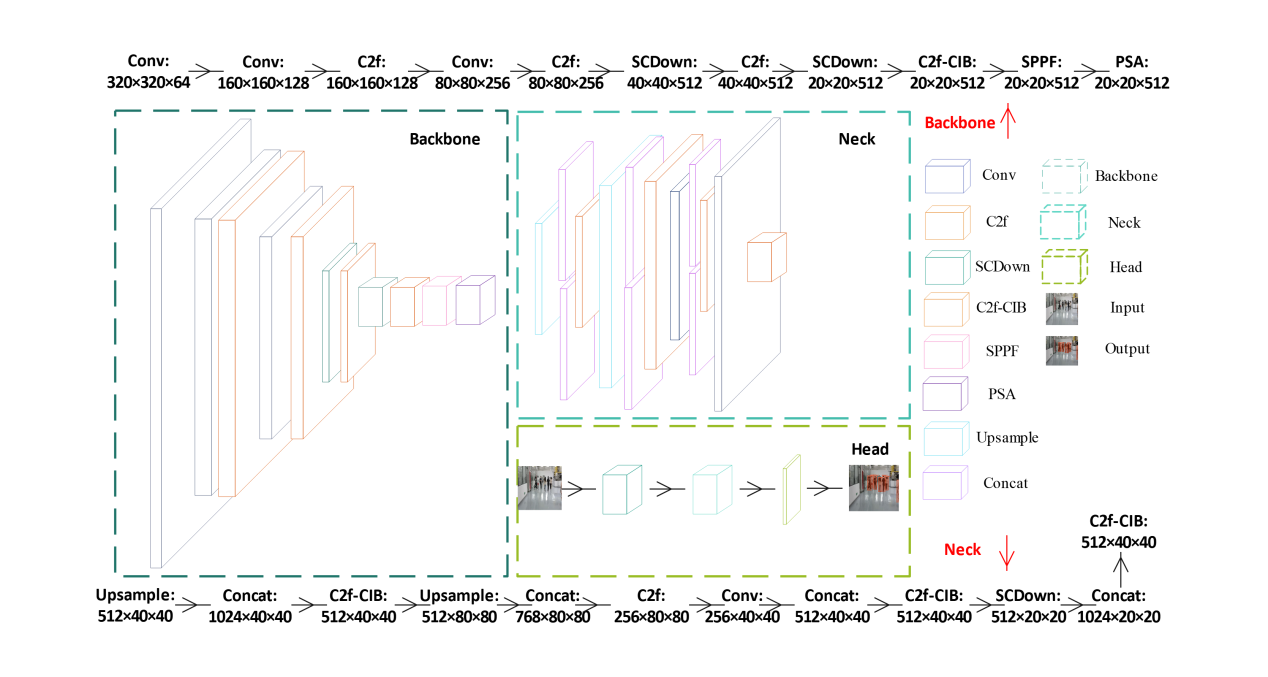
\includegraphics[width=1.0\textwidth]{fig0032.png}  % Replace "example-image" with the file name of your image
	\caption{Deep Learning and Neural Networks}
	\label{fig:0032}
\end{figure}

\subsection*{The Mid-term Report and Future Plans}

In this week’s mid-term report, we outlined our progress and demonstrated how our fine-tuned model has improved translation accuracy. So far, we’ve managed to achieve \textbf{a BLEU score of 74.6}, which indicates that our translations are closely aligned with the human-generated reference translations. However, we are far from finished. There’s always room for improvement, particularly when it comes to translating more complex mathematical expressions.

As we move forward, we plan to continue fine-tuning the model, focusing particularly on:
\begin{itemize}
	\item \textbf{Incorporating the term dictionary}: This will further reduce errors in terminology and improve consistency.
	\item \textbf{Data augmentation}: We plan to increase our dataset size by introducing more variations of the same text, which will improve the model’s ability to generalize.
	\item \textbf{Data augmentation}: We plan to increase our dataset size by introducing more variations of the same text, which will improve the model’s ability to generalize.
	\item \textbf{Multimodal learning}: Our future work will explore ways to handle both text and formulas more seamlessly.
\end{itemize}

\subsection*{Conclusion}

In conclusion, this week has been both a reflection of our progress and a realization of the challenges ahead. The mid-term report was a crucial milestone, but it also highlighted areas that need further refinement. The journey of fine-tuning a large model for mathematical textbook translation has been intellectually rewarding, but the road ahead will require persistence and innovation. For now, I remain optimistic that our project will achieve its goals, and I look forward to the breakthroughs that the next few months will bring.

\section{Week 6 Diary: Design of an Intelligent Logistics Vehicle}

This week, I had the opportunity to participate in an engineering practice competition where the task was to design an intelligent logistics vehicle. As someone who has always been fascinated by automation and robotics, this project felt like a perfect fit. However, little did I know that turning a concept into a functional vehicle would involve navigating a maze of electronics, coding, and logistical challenges. Spoiler alert: it wasn’t easy, but it was incredibly rewarding.

\subsection*{The Concept Behind the Intelligent Logistics Vehicle}

The goal of our project was to develop a vehicle capable of automating the transportation of goods within a warehouse setting. The vehicle had to navigate autonomously, avoiding obstacles, following a designated path, and picking up and delivering items without human intervention. The design was inspired by real-world applications in logistics and manufacturing, where efficiency and accuracy are critical.

To achieve this, we integrated several key technologies:
\begin{itemize}
	\item \textbf{Stepping motors}: These motors allowed us to control the precise movement of the vehicle, adjusting speed and direction smoothly.
	\item \textbf{Sensors}: Ultrasonic and infrared sensors were used to detect obstacles and ensure that the vehicle could navigate through complex environments.
	\item \textbf{CAN communication}: To handle the various modules, we utilized the Controller Area Network (CAN) protocol, which enabled the different parts of the vehicle to communicate seamlessly.
	\item \textbf{Autonomous navigation algorithms}: We implemented path-planning algorithms that enabled the vehicle to find the shortest route and avoid collisions.
\end{itemize}

\begin{figure}[h!]
	\centering
	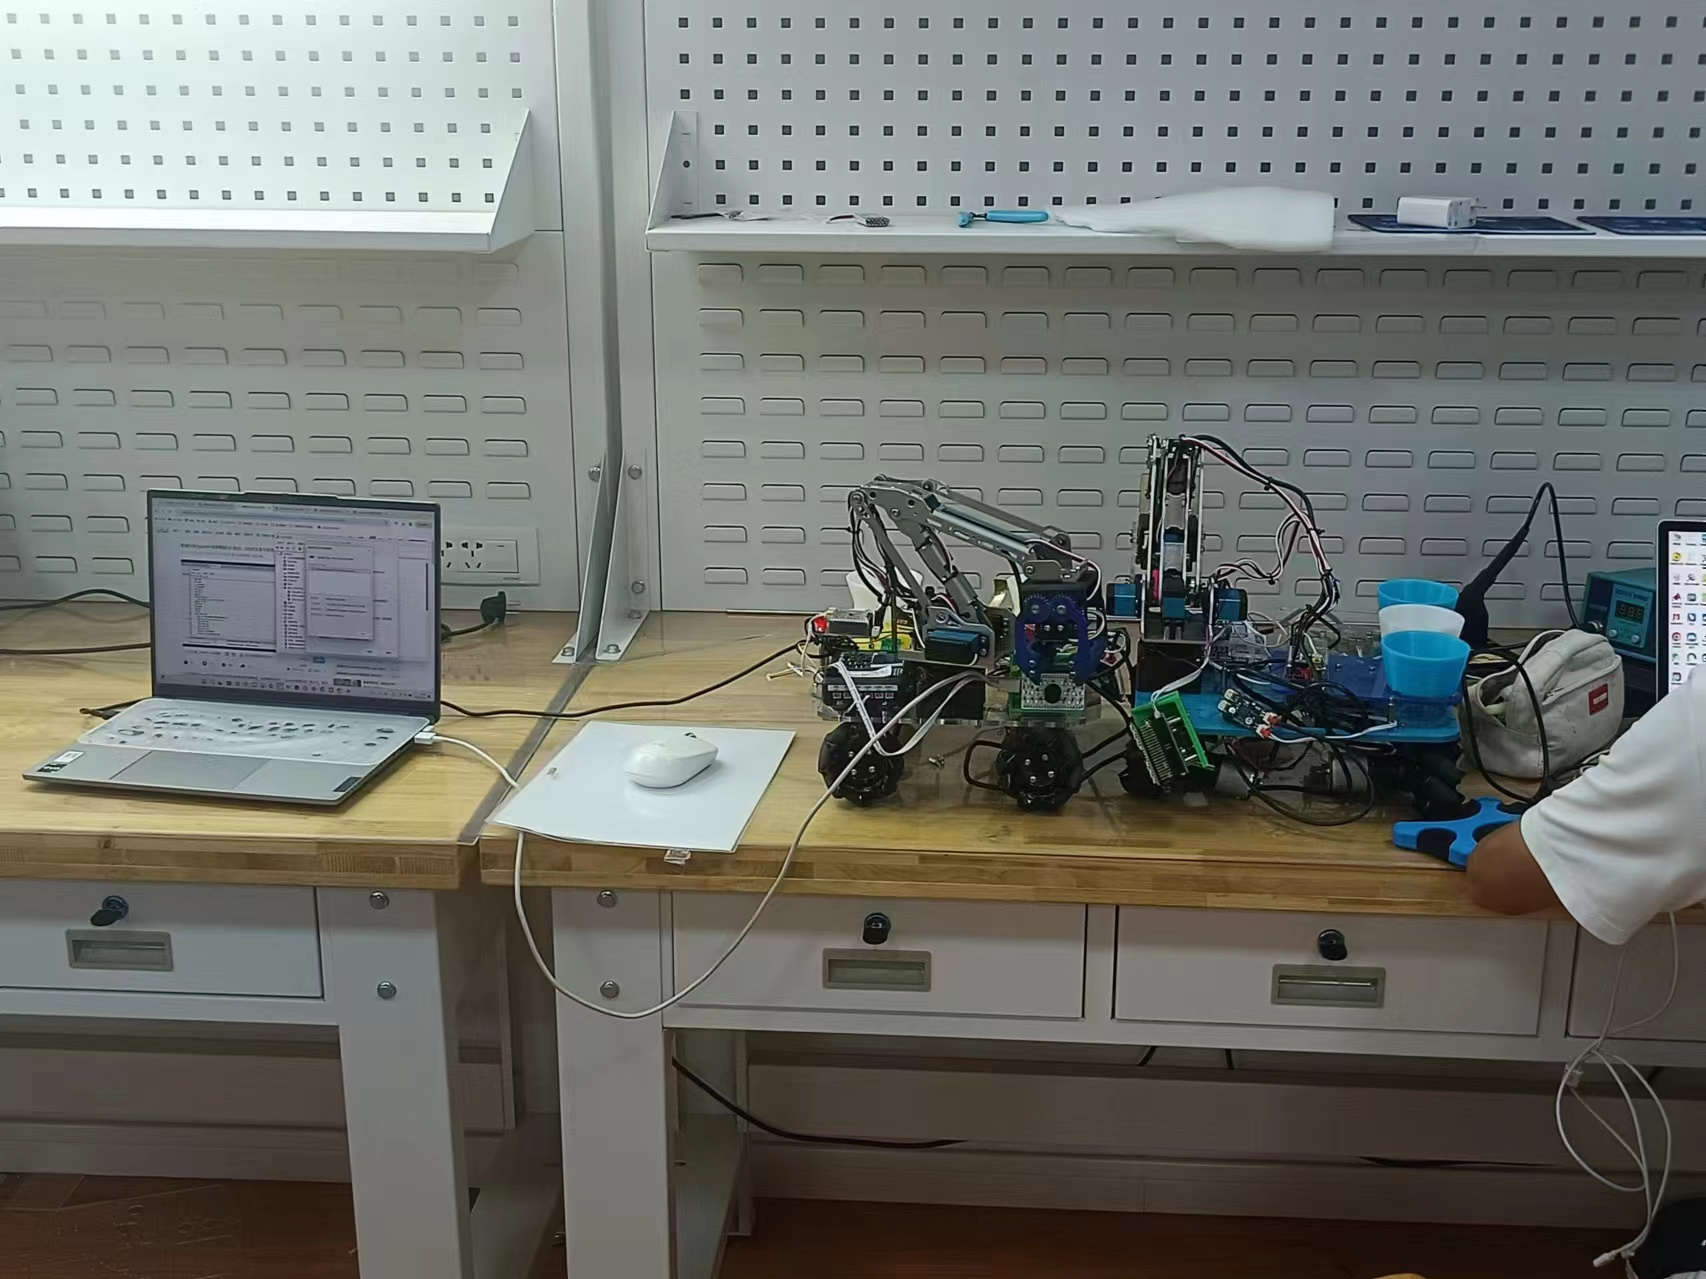
\includegraphics[width=0.8\textwidth]{fig005.jpg}  % Replace "example-image" with the file name of your image
	\caption{Intelligent logistics vehicle}
	\label{fig:005}
\end{figure}

\subsection*{The Challenges of Designing and Testing the Vehicle}

Building the vehicle was no small task. It involved a delicate balance of hardware integration and software development. One of the biggest challenges was ensuring that the stepping motors worked in perfect sync with the sensors and navigation algorithms. As mentioned in the documentation

$\&$8203;:contentReference[oaicite:0]{index=0}

$\&$8203;:contentReference[oaicite:1]\{index=1\}

$\&$8203;:contentReference[oaicite:2]\{index=2\}

managing the CAN communication between the control units and the motors required meticulous calibration. Each module had to be fine-tuned to ensure that the vehicle could move smoothly and stop precisely at the designated points.

One memorable moment was when the vehicle, instead of stopping at the drop-off point, decided to take a scenic tour of the workshop. It turned out that the issue was a miscalibrated sensor. After several attempts at debugging, including reconfiguring the motor control settings

$\&$8203;:contentReference[oaicite:3]\{index=3\}, we finally got it right. The sense of accomplishment when the vehicle performed perfectly was worth all the effort (and frustration).

\subsection*{Software Development and Debugging Nightmare}

The software side of the project also had its fair share of challenges. Programming the vehicle’s logic—especially the decision-making algorithms for obstacle avoidance and path planning—proved to be more complex than expected. We utilized the popular \textbf{STM32 microcontroller} as the vehicle’s brain and wrote the control logic in C. The code itself wasn’t overly complicated, but debugging was another story.

There were several instances where I found myself staring at a screen full of code, wondering why nothing seemed to work. As it turns out, even small mistakes in sensor calibration or CAN protocol communication could cause the entire system to malfunction. After countless hours of testing and debugging, the system finally reached a stable state.

\subsection*{Lessons Learned and Looking Ahead}

This project taught me a lot about the intricacies of designing an autonomous system, from hardware integration to software debugging. One of the key takeaways was the importance of rigorous testing and calibration. Even the most advanced algorithms are only as good as the sensors and motors they control. Misaligned components can lead to unexpected (and sometimes hilarious) results.

Looking ahead, I am excited to continue refining the vehicle’s design and functionality. The competition may be over, but there is always room for improvement. I hope to apply what I’ve learned to future projects, especially in the field of robotics and autonomous systems.

\subsection*{Conclusion}

In conclusion, the design of the intelligent logistics vehicle was a challenging but rewarding experience. From stepping motor calibration to CAN communication and autonomous navigation, the project pushed me to explore new technical areas and hone my problem-solving skills. While there were moments of frustration, the final product—a vehicle that could autonomously navigate and transport goods—made all the effort worthwhile. I look forward to building on this foundation in future competitions and projects.



\section{Week 7 Diary: Reading Agatha Christie’s Detective Classics}

This week, I embarked on a literary journey that transported me into the intriguing and, dare I say, ominous world of Agatha Christie. I devoured three of her most iconic works: **The ABC Murders**, **Murder on the Orient Express**, and **And Then There Were None**. As I delved deeper into these narratives, I found myself not merely reading them, but becoming subtly entangled in the intricate web of mystery and suspicion. By the end, I couldn't shake off the feeling that I, too, might be a character in some grand conspiracy—perhaps one of Christie's own making.

\subsection*{The ABC Murders: Alphabetical Anarchy}

Starting with **The ABC Murders**, I was immediately drawn in by the calculated precision with which the killer chose his victims. The methodical, almost mechanical selection of victims based on their names and locations gave the crime spree an unsettling sense of order amid the chaos. Hercule Poirot, with his signature poise, navigated through the clues with finesse, while I, in stark contrast, felt like a flustered amateur detective struggling to keep up.

As the plot thickened, it became apparent that Christie was playing a psychological game—not only with Poirot but also with the reader. The subtle red herrings, the apparent randomness of the killings, and the ultimate revelation that the entire case was a ruse all contributed to the feeling that I, too, had been masterfully misled. By the time I finished the book, I couldn't help but wonder if my own life was a series of cleverly disguised patterns that I had yet to decipher.

\subsection*{Murder on the Orient Express: A Train Full of Secrets}

Next, I tackled **Murder on the Orient Express**, a novel that presents a seemingly impossible crime: a murder committed in a locked train compartment with no obvious suspects. What unfolds is a classic "whodunit" where every passenger has a motive, yet none seem likely to be the culprit. Once again, Poirot steps in to unravel the mystery, this time uncovering a truth so unexpected and shocking that it redefines the very nature of justice.

What fascinated me most about this novel was the moral ambiguity. The conclusion—that every passenger had a hand in the murder—raised profound questions about collective guilt and the limits of the law. By the time Poirot reveals the truth, I was no longer simply a passive reader but an active participant in the ethical dilemma. Should the passengers be punished for their crime, or was their act of retribution justified? These questions lingered long after I closed the book, leaving me with the unsettling feeling that sometimes, justice is as complex and multifaceted as the crimes it seeks to punish.

\begin{figure}[h!]
	\centering
	
\includegraphics[width=0.3\textwidth]{fig006.jpg}  % Replace "example-image" with the file name of your image
	\caption{insight}
	\label{fig:006}
\end{figure}

\subsection*{And Then There Were None: Isolation and Suspicion}

Lastly, I dove into **And Then There Were None**, a novel that left me genuinely unnerved. The story’s premise—ten strangers invited to a remote island, only to be picked off one by one—felt like an inescapable nightmare. With no detective to save the day, the characters (and I, by extension) were left to their own devices, trapped in a deadly game of survival.

What struck me was the psychological toll of isolation and suspicion. As each character met their demise, the sense of paranoia grew, until it became impossible to distinguish friend from foe. The clever use of the "Ten Little Soldiers" nursery rhyme as a blueprint for the murders only heightened the tension. By the end, I found myself glancing over my shoulder, wondering if perhaps I, too, was being watched, judged, and marked for an inevitable fate.

\subsection*{The Grand Conspiracy}

Having finished all three novels, I can't shake off the feeling that I've been drawn into something larger than myself. Each of these stories played with my sense of reality, making me question the motives of everyone around me. It’s as though Christie herself is whispering in my ear, urging me to look for hidden clues in everyday life. Perhaps the world is, after all, a grand conspiracy—one that I have only begun to understand.

\subsection*{Conclusion}

In conclusion, my week spent with Agatha Christie’s works has been as thrilling as it has been intellectually stimulating. Through her masterful storytelling, Christie not only entertained me but also made me reflect on the nature of truth, justice, and human behavior. The subtle sense of being pulled into a grand conspiracy persists, and I can't help but wonder—could this be the true genius of Christie’s work? To leave her readers questioning not only the mysteries within the pages but the mysteries of life itself?

\section{Week 8 Diary: Preparing for Midterm Exams}

This week, I found myself facing the most formidable academic challenge of the semester so far: the midterm exams. With five courses demanding attention—\textbf{Materials Mechanics}, \textbf{Mechanical Principles}, \textbf{Probability Theory and Mathematical Statistics}, \textbf{Mechanical Engineering Materials}, and \textbf{Mechanical Drawing}—the pressure is on. It's a cocktail of stress, late-night study sessions, and an ever-growing pile of lecture notes. Yet, amid the chaos, there’s a strange sense of satisfaction. The struggle, after all, is part of the process. Painful? Yes. Rewarding? Also, yes.

\subsection*{Materials Mechanics: The Stress-Strain of My Life}

Let's start with \textbf{Materials Mechanics}, a subject that feels strangely poetic at times. Stress and strain, tension and compression—these terms are not just confined to the materials we study, but seem to perfectly describe my own emotional state as the exam approaches. The equations, though daunting, have a rhythm to them, and once I understand the mechanics behind them, they actually start to make sense. 

However, the challenge comes from the countless derivations and formulas I need to remember. It's as if every problem introduces a new twist or boundary condition, just to keep me on my toes. After hours of practice, I've learned that Materials Mechanics is not just about memorizing formulas but understanding the principles behind them. Still, there are moments when I feel like the very beams and supports I’m studying are about to buckle—along with my brain.

\subsection*{Mechanical Principles: Gears, Cams, and Complicated Diagrams}

Next up is \textbf{Mechanical Principles}, which might as well be called "How to Make Things Move—For Real." Here, gears and cams rule the day, and understanding the motion of machines is both fascinating and frustrating. The hardest part? The diagrams. Oh, the diagrams. It’s not enough to understand the theory; I also need to be able to draw and interpret complex mechanical systems on the fly.

But there’s a certain satisfaction in finally getting it right—when the gears align, both figuratively and literally. The satisfaction of solving a complex motion problem is akin to watching a well-oiled machine in action. It’s a lot of work, but when things click into place, the feeling is worth it.

\subsection*{Probability Theory and Mathematical Statistics: Rolling the Dice}

As if the mechanical courses weren’t enough, there’s also \textbf{Probability Theory and Mathematical Statistics}. This subject feels like an intellectual workout. At times, it’s like rolling the dice and trying to predict the outcome, while at other times, it’s about making sense of data and drawing conclusions from it. 

The tricky part of this course is balancing the theoretical aspects with practical applications. Understanding the nuances of distributions, hypothesis testing, and the infamous central limit theorem requires both mathematical rigor and intuition. Despite the complexity, there’s something strangely addictive about solving probability problems. Maybe it’s the uncertainty of it all that keeps me going. After all, who doesn’t love a little unpredictability?

\subsection*{Mechanical Engineering Materials: The Science of Strength}

\textbf{Mechanical Engineering Materials} is another beast entirely. It’s all about the materials that make up the machines and structures we rely on every day. From metals to polymers, ceramics to composites, understanding their properties—strength, ductility, hardness, and toughness—requires a deep dive into the science of materials.

What makes this subject challenging is not just the breadth of content but the need to apply these properties to real-world scenarios. Why does one material perform better under certain conditions than another? And how do we select the right material for the job? These are the questions that haunt my study sessions, but also motivate me to push through the dense content.

\subsection*{Mechanical Drawing: Drawing My Way Through the Exam}

Finally, there’s \textbf{Mechanical Drawing}, where precision is key. Whether it’s a detailed sketch of a gear assembly or a complex cross-sectional view, everything must be perfectly aligned, labeled, and dimensioned. One wrong line, and the entire diagram could be misunderstood.

While I’ve always enjoyed drawing, doing so under exam conditions is a different story. The clock is ticking, and each line needs to be exact. Still, there’s a sense of calm in the precision required, as though the act of drawing helps bring order to the chaos of exam preparation.

\subsection*{Conclusion: Painful but Worth It}

In conclusion, preparing for these midterm exams has been both a mental and physical endurance test. From stress-strain analysis to complex probability calculations, each subject has its own unique demands. Yet, despite the long hours and occasional frustration, I can’t help but feel a sense of accomplishment. Painful as it may be, there’s no better feeling than seeing hard work pay off. Now, all that’s left is to tackle the exams head-on—and maybe treat myself to a well-deserved break afterward.


\section{Week 9 Diary: Learning SolidWorks and AutoCAD for Mechanical Simulation and Drafting}

This week has been all about diving deep into the world of mechanical simulation and drafting with two powerful software tools: \textbf{SolidWorks} and \textbf{AutoCAD}. As someone who is relatively new to the intricacies of mechanical design, I found myself simultaneously fascinated and overwhelmed by the sheer possibilities that these programs offer. Between sketching models, simulating movements, and generating technical drawings, this week was both a challenge and a joy—a perfect blend of precision, creativity, and problem-solving.

\subsection*{SolidWorks: Building the Future, One Part at a Time}

SolidWorks is, without a doubt, one of the most comprehensive tools for mechanical simulation and 3D modeling. From the moment I opened the program, I was greeted with a dizzying array of features—tools for creating parts, assemblies, simulations, and drawings. At first, it felt a bit like stepping into a vast, unfamiliar workshop where every tool is shiny but slightly intimidating.

But once I got the hang of it, things began to fall into place. My first task was to design a simple mechanical part—a bracket. What began as a basic 2D sketch soon morphed into a fully-fledged 3D model as I learned to extrude, cut, and fillet edges. The process was surprisingly intuitive, and there was something immensely satisfying about seeing the flat sketch on my screen turn into a real, tangible object (even if it only existed in virtual form).

One of the highlights of the week was using the \textbf{simulation features}. I was able to test how my bracket would hold up under different stress conditions, something that’s crucial in mechanical engineering. It turns out, seeing your model bend and deform under simulated loads is both terrifying and exhilarating. It’s like watching a suspenseful thriller, except the plot twist involves finding out whether or not your design can withstand the real-world forces it’s supposed to handle!

\begin{figure}[h!]
	\centering
	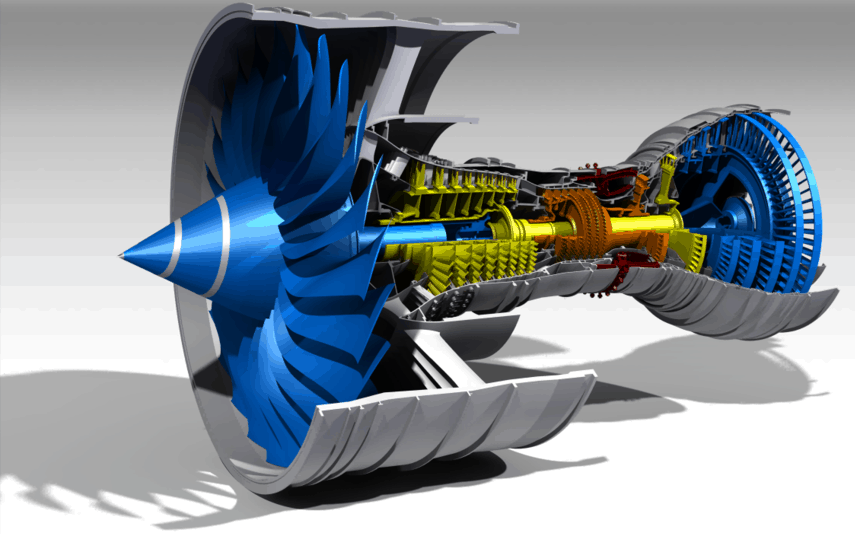
\includegraphics[width=0.8\textwidth]{fig007.png}  % Replace "example-image" with the file name of your image
	\caption{3D Solidworks}
	\label{fig:007}
\end{figure}

\subsection*{AutoCAD: Mastering the Art of Precision}

On the other side of the spectrum is \textbf{AutoCAD}, which focuses more on 2D drafting and precision. Compared to SolidWorks, AutoCAD feels like the no-nonsense, highly disciplined older sibling. Every line, every curve, every dimension has to be perfect—and AutoCAD makes sure you’re aware of that. There’s no room for guesswork here.

My introduction to AutoCAD involved learning the fundamentals of technical drawing. This includes drafting orthographic views, section views, and detailed dimensions of mechanical parts. While SolidWorks excels at giving a tangible sense of the 3D form, AutoCAD drills down to the details—ensuring that every aspect of a mechanical component is represented with precision.

At first, I found myself struggling with the grid system, snapping features, and commands like "\textbf{Offset}", "\textbf{Trim}", and "\textbf{Chamfer}". But as I practiced, the workflow became smoother, and I began to appreciate AutoCAD’s methodical approach. The satisfaction of creating a perfectly dimensioned drawing, where every millimeter counts, cannot be overstated. It’s a bit like doing a puzzle where every piece has to fit exactly—frustrating at times, but immensely rewarding when everything comes together.

\subsection*{Mechanical Drawing: Bringing the Two Worlds Together}

What’s fascinating about using both SolidWorks and AutoCAD is how they complement each other. SolidWorks allows me to visualize, simulate, and build a model, while AutoCAD ensures that the technical drawings are precise and accurate. In the real world, both the 3D model and the 2D technical drawing are crucial for manufacturing and assembly. Together, they form the blueprint for turning an idea into a functional machine or structure.

This week’s focus on mechanical drawing has taught me a lot about the importance of communication in engineering. A brilliant design is worthless if it can’t be properly communicated to the people responsible for manufacturing it. SolidWorks and AutoCAD serve as the bridge between the engineer’s mind and the hands that bring the design to life.

\subsection*{A Glimpse into the Future of Mechanical Engineering}

As I continue to explore these tools, I can’t help but imagine the endless possibilities they open up. Whether it’s designing complex machines, simulating stress and movement, or creating technical drawings that can be sent straight to a manufacturing plant, SolidWorks and AutoCAD are essential in modern engineering. While I still have much to learn, this week has given me a strong foundation to build on—and I’m excited to see where this knowledge will take me in future projects.

\subsection*{Conclusion}

In conclusion, learning SolidWorks and AutoCAD has been both challenging and rewarding. Each software offers a unique approach to mechanical design—one focused on 3D modeling and simulation, the other on precise technical drafting. While mastering these tools takes time and effort, the sense of accomplishment that comes from creating and testing designs is incredibly fulfilling. I look forward to continuing this journey into the world of mechanical engineering, one part at a time.

\section{Week 10 Diary: Advanced Mathematics Competition}

This week, I had the honor (and perhaps the misfortune) of participating in the **Advanced Mathematics Competition**. From the moment I sat down and looked at the exam paper, I realized this wasn’t going to be a stroll in the park. The competition tested us on a wide range of advanced mathematical topics: limits, the mean value theorem, Lagrange interpolation, solving differential equations, surface integrals of multivariable functions, Euler’s number, Stirling’s formula, and many others that I’d probably prefer to forget for now. To say it was challenging would be an understatement. 

\subsection*{Limits and the Mean Value Theorem: The Warm-up}

The first few questions were centered around **limits** and the **mean value theorem**. It felt like a decent warm-up, but I quickly realized that even these “basic” concepts were being tested in tricky ways. The questions were designed to push the boundaries of my understanding of these fundamental ideas. What seemed like straightforward limits turned out to have hidden subtleties that made me question my methods. And the mean value theorem, while conceptually simple, was applied in such convoluted ways that I found myself double-checking every step, unsure if I had truly grasped the core idea.

\subsection*{Lagrange Interpolation: Not as Simple as It Sounds}

One of the later questions tested my knowledge of **Lagrange interpolation**. In theory, this method of constructing a polynomial that passes through a given set of points isn’t too hard to understand. But under the pressure of the competition, with time ticking away, even writing down the interpolation formula felt like solving a complex puzzle. Finding the interpolating polynomial wasn’t the hard part—the real challenge was avoiding the numerous traps set by the question, where one small mistake could send the entire solution off course.

\subsection*{Differential Equations: Solving or Surrendering?}

Then came the **differential equations**, a topic that can either be beautifully elegant or horrifically complex depending on the specific equation at hand. Of course, the competition leaned towards the latter. The differential equations we were tasked with solving required a mix of creativity and perseverance. While I tried my best to recall the various techniques—separation of variables, integrating factors, and characteristic equations—I couldn’t help but feel like I was fighting a losing battle. By the time I finished solving the differential equations, I wasn’t entirely sure if I had found the correct solution or just something that looked reasonable on paper.

\subsection*{Multivariable Calculus and Surface Integrals: A Different Dimension of Difficulty}

Moving on to **surface integrals of multivariable functions**, I quickly realized that my earlier confidence in double and triple integrals was not as robust as I thought. Surface integrals bring in a whole new dimension of difficulty, both literally and figuratively. Visualizing the surfaces in question, setting up the integral bounds, and actually performing the integration—each step was an uphill struggle. I found myself staring at the equations, hoping for some sort of breakthrough that would make everything click. Alas, that breakthrough didn’t come, and I left the surface integrals section feeling rather defeated.

\subsection*{Euler’s Number and Stirling’s Formula: The Final Blow}

As if things weren’t difficult enough, the final questions dealt with **Euler’s number** and **Stirling’s formula**. These topics, often seen in the context of limits, infinite series, and approximations, are beautiful in their own right. But during an exam, when the pressure is on, beauty tends to take a backseat to panic. Stirling’s approximation, in particular, requires careful handling, and it felt as though every calculation I made had the potential to go horribly wrong at any moment. I tried to remain calm, but by this point, I couldn’t shake the feeling that my performance was far from ideal.

\subsection*{A Humbling Experience}

In the end, I left the competition with mixed feelings. On the one hand, I was proud to have participated and challenged myself with such high-level mathematics. On the other hand, I couldn’t help but feel like I hadn’t performed to the best of my abilities. Perhaps it was the pressure, the time constraints, or just the sheer difficulty of the questions, but something about the competition left me feeling humbled. Mathematics, it seems, has a way of keeping us grounded, no matter how much we think we know.

\subsection*{Conclusion}

In conclusion, the Advanced Mathematics Competition was an eye-opening experience. It reminded me that even the concepts we think we understand can become daunting when presented in new and unfamiliar ways. From limits to Euler’s number, each question pushed me to my limits, both intellectually and emotionally. While I may not have achieved a perfect score, I gained something even more valuable: a deeper respect for the complexity and beauty of mathematics. Now, I just hope that my results reflect some of the hard work I’ve put in!

\section{Week 11 Diary: Turning 20 - Reflections on My Birthday}

This week marked a significant milestone in my life—I turned 20 years old. As I celebrated my birthday, I found myself reflecting on the transition from teenage years to adulthood, a process that feels both exciting and, admittedly, a little daunting. It’s strange to think that I am now two decades old, and as much as I would like to say that I have everything figured out, the reality is far more complex.

\subsection*{The Joy of Turning 20: A New Chapter}

Turning 20 comes with its own unique sense of joy. No longer a teenager, I feel as though I’ve entered a new chapter of life, one filled with opportunities for growth, learning, and self-discovery. My birthday was a simple affair, celebrated with close friends and family, but it was filled with warmth and affection. There’s something about the beginning of a new decade that makes me feel as though the world is full of possibilities, and the future—while uncertain—seems full of promise.

Reaching this milestone has also given me the chance to reflect on the past. Looking back, I see how much I’ve grown, both personally and academically. The challenges I’ve faced and the successes I’ve enjoyed over the years have shaped me into the person I am today. From navigating the complexities of university life to preparing for academic competitions, each experience has contributed to my development. At the same time, turning 20 makes me realize how much more there is to learn and how many more experiences lie ahead.

\begin{figure}[h!]
	\centering
	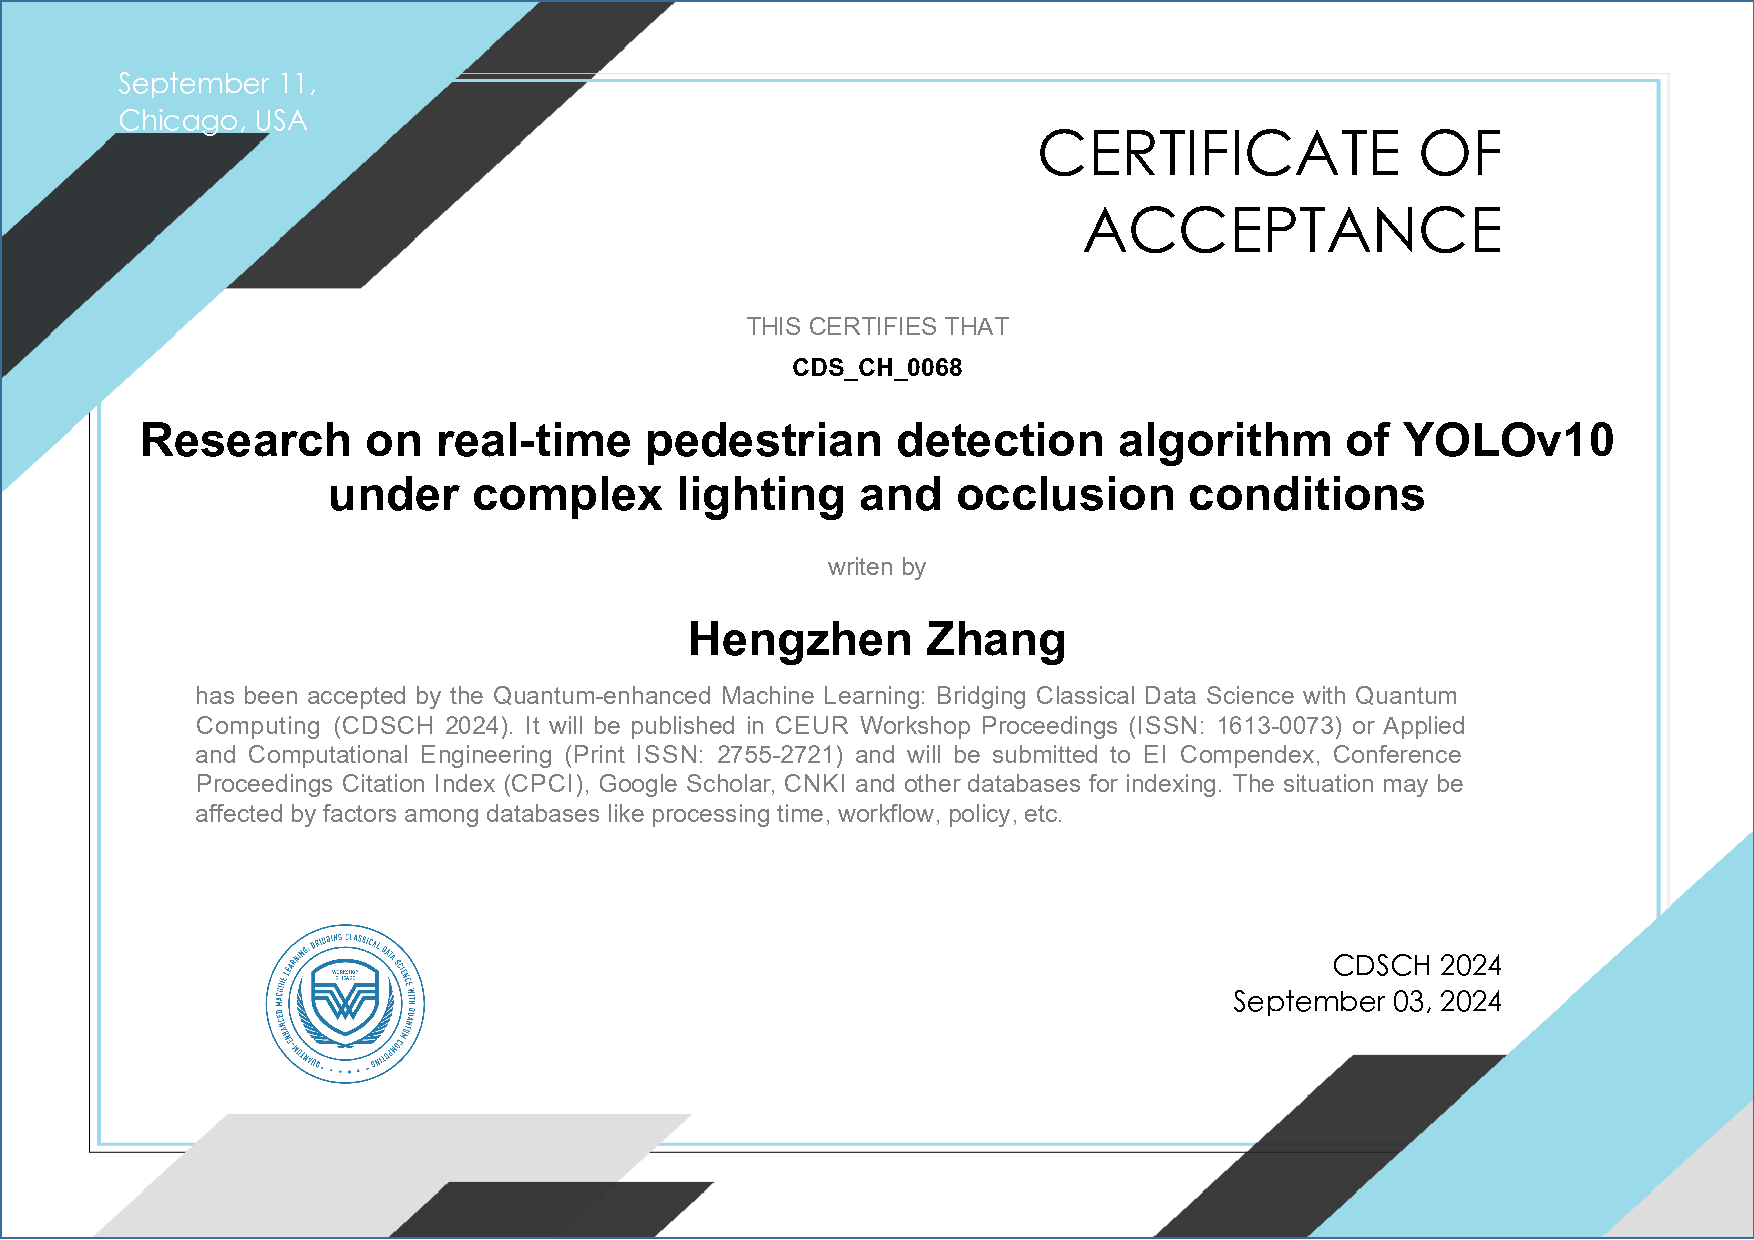
\includegraphics[width=0.8\textwidth]{fig0030.pdf}  % Replace "example-image" with the file name of your image
	\caption{My independently written paper has been accepted}
	\label{fig:0030}
\end{figure}

\subsection*{Growth and Self-Discovery: The Path Forward}

With this milestone comes a greater awareness of the responsibilities and opportunities that adulthood brings. In many ways, I feel more confident than ever before. I’ve spent the last few years laying the foundation for my future, and now it feels like the time to build upon it. Whether it’s through furthering my education, engaging in new projects, or simply exploring new interests, the possibilities are endless.

However, with growth comes the inevitable feeling of uncertainty. Turning 20 has made me think more deeply about the future—about my career, my goals, and the kind of person I want to become. While I have a sense of direction, there are still so many unknowns. What if the path I’ve chosen isn’t the right one? What if my interests change along the way? These questions linger in my mind, but I remind myself that uncertainty is a natural part of life. In fact, it’s often in moments of uncertainty that the greatest opportunities for growth and self-discovery arise.

\subsection*{Life Lessons and a Positive Attitude}

As I step into my 20s, I’ve come to realize that a positive attitude is key to navigating life’s ups and downs. Life will inevitably throw challenges my way—whether they come in the form of academic pressures, personal dilemmas, or career decisions. But I’ve learned that maintaining a sense of optimism, even in the face of difficulties, can make all the difference.

One of the greatest lessons I’ve learned is that growth doesn’t always come in a straight line. Sometimes, the most valuable experiences come from the unexpected detours. In this sense, turning 20 isn’t just about leaving behind my teenage years—it’s about embracing the unknown and being open to whatever comes next. I’ve also realized that it’s okay not to have all the answers. After all, part of the excitement of life is figuring things out along the way.

\subsection*{The Road Ahead: Balancing Ambition and Uncertainty}

As I look toward the future, I’m filled with a mix of excitement and a healthy dose of anxiety. The road ahead is filled with potential, but it’s also marked by uncertainty. What will my career look like? Where will my passions lead me? These questions don’t have clear answers yet, but I’m learning to be comfortable with that.

For now, I’m focusing on continuing to learn, grow, and take advantage of the opportunities that come my way. Whether it’s furthering my studies, pursuing new projects, or simply taking the time to enjoy the present moment, I’m determined to make the most of my 20s. While the journey ahead may be unpredictable, I know that with a positive attitude and an open mind, I’ll be ready to face whatever comes my way.

\subsection*{Conclusion}

In conclusion, turning 20 has been a time of reflection, growth, and anticipation. While I still have much to learn and many uncertainties to face, I’m optimistic about the future and excited for the challenges and opportunities that lie ahead. The next chapter of my life is just beginning, and I’m ready to embrace it with a sense of curiosity and adventure.

\section{Week 12 Diary: Preparing for the CET-6 Exam}

As the CET-6 English exam approaches, I find myself navigating through a mix of emotions—anxiety, determination, and a faint glimmer of hope. Preparing for such a challenging exam feels like running a marathon, but with the added twist of attempting to decipher English accents and grammar rules along the way. English has always been one of those subjects that I both admire and struggle with. And this week, as I ramp up my preparation, it feels as though the difficulty of the exam is amplifying with every practice test.

\subsection*{The Listening Section: My Arch-nemesis}

Let’s start with the obvious challenge: \textbf{listening}. The listening section of CET-6 is, in one word, brutal. There’s something uniquely stressful about trying to keep up with fast-paced conversations, academic lectures, and all sorts of accents—some of which seem to be designed to confuse rather than to communicate. I can’t tell you how many times I’ve been halfway through a listening exercise, only to realize that I’ve missed an entire question because I was still mentally processing the previous sentence.

My typical reaction to the listening section goes something like this: the audio begins, I confidently jot down the first answer, and then suddenly—chaos. As the voices continue, my mind races to catch up. By the time I’ve figured out what one speaker said, I’ve missed the next few lines. It’s as though the conversation is happening on fast forward, while my comprehension is stuck on pause.

Despite the challenges, I’ve been diligently practicing. \textbf{Mock tests}, \textbf{listening drills}, and even \textbf{watching English shows} have become part of my daily routine. I’ve learned to focus on key words, and I’ve become more familiar with the types of questions that usually appear. But no matter how much I practice, the listening section always feels like a guessing game. I just hope that on the day of the exam, my guessing skills are sharp.

\subsection*{Reading and Writing: Familiar but Formidable}

While listening feels like the trickiest part, the \textbf{reading} and \textbf{writing} sections are not without their own set of difficulties. The reading comprehension questions require both speed and accuracy, which is a challenge when faced with complex passages filled with advanced vocabulary and subtle nuances. Every time I read an article, I find myself second-guessing the true meaning behind every sentence. Is the author hinting at something deeper? Or is it just a straightforward statement? The pressure to pick the right answer weighs on me as I navigate through the passages.

As for \textbf{writing}, well, I’ve always enjoyed it more than listening or reading. But writing for an exam like CET-6 comes with its own unique pressure. The essay topics are broad, often requiring a sophisticated understanding of global issues or abstract concepts. It’s not just about having good grammar—it’s about crafting an argument, presenting ideas logically, and all within a limited time. I’ve been practicing by writing essays on various topics, but I can’t help but feel that my vocabulary sometimes limits my ability to express my thoughts as clearly as I would like.

\subsection*{Brushing Up on Vocabulary: A Never-Ending Battle}

Ah, \textbf{vocabulary}—the foundation of any language. Unfortunately, my relationship with English vocabulary has been rocky. For every new word I learn, it seems like I forget two others. CET-6 has a reputation for testing not just everyday English but also academic and formal vocabulary. As I go through my flashcards, I’m constantly reminded of how vast the English language truly is.

My strategy has been to focus on high-frequency words and idiomatic expressions that commonly appear in past exams. I’ve also started reading more English articles, which helps reinforce the vocabulary in context. But let’s be honest—there’s only so much my brain can absorb in a short period of time. Still, I remain optimistic that all these hours of memorization will pay off in the end.

\subsection*{Hopeful Yet Realistic: The Final Countdown}

With the exam just around the corner, I’m trying to strike a balance between hope and realism. On one hand, I’ve put in a lot of effort—practicing listening, reading challenging articles, expanding my vocabulary, and writing essays under timed conditions. On the other hand, I know that CET-6 is a tough exam, and there’s a chance that my performance won’t be perfect.

But that’s okay. I’ve come to realize that exams are not just about the score—they’re about the process of learning, improving, and challenging myself. Regardless of the result, I’m proud of the effort I’ve put in. If nothing else, preparing for CET-6 has improved my overall English skills, and that’s something I can carry forward beyond the exam room.

\subsection*{Conclusion}

In conclusion, preparing for CET-6 has been both a frustrating and rewarding experience. From struggling with the listening section to building my vocabulary, I’ve faced challenges at every step. But I’ve also grown as a language learner, and I’m hopeful that my hard work will be reflected in my final score. For now, all I can do is keep practicing, stay focused, and hope for the best on exam day.

\section{Week 13 Diary: SITP Defense of Heavy Vehicle Carbon Emission Model}

This week marked an important milestone in our \textbf{Student Innovation and Technology Program (SITP)}, where my team and I presented and defended our project on \textbf{heavy vehicle carbon emission prediction}. It was a thrilling experience—equal parts nerve-wracking and satisfying—culminating in months of hard work where we merged cutting-edge \textbf{deep learning} techniques with \textbf{vehicle dynamics modeling} to predict carbon emissions.

Given the global focus on reducing carbon emissions and achieving net-zero goals, this project was more than just an academic exercise. It felt like a small but meaningful contribution to the grander goal of green development, particularly in the context of the \textbf{dual-carbon} targets that have been set worldwide.

\subsection*{The Core of the Model: LSTM-GRU Hybrid and ARIMA}

Our model leveraged both \textbf{deep learning} and \textbf{traditional time series approaches}. At its heart was a \textbf{LSTM-GRU hybrid model}, which we chose for its ability to capture long-term dependencies in sequential data, particularly time-series data like vehicle operation metrics. The \textbf{LSTM (Long Short-Term Memory)} component allowed us to effectively manage the long-term dependencies in carbon emissions patterns, while the \textbf{GRU (Gated Recurrent Unit)} helped simplify the model’s complexity and speed up the learning process.

However, we didn’t stop there. Alongside this hybrid model, we integrated \textbf{ARIMA (AutoRegressive Integrated Moving Average)} for time series forecasting, especially for short-term carbon emission prediction. The ARIMA model excelled at handling data that showed clear trends and seasonality, which was important for our analysis of carbon emissions under varying operating conditions.

To round off our approach, we also experimented with a \textbf{Prohibit model} for certain scenarios where discrete restrictions on emissions were necessary, though this was more of a backup model in case we encountered specific constraints during predictions.

\subsection*{The Role of Vehicle Dynamics: A Physical Layer to the Prediction}

While deep learning is powerful, we wanted to ensure that our model was grounded in the real-world mechanics of heavy vehicles. That’s where the \textbf{vehicle dynamics modeling} came into play. Using a physics-based approach, we accounted for factors like vehicle weight, engine efficiency, fuel consumption, and load distribution. These physical dynamics provided a layer of realism to our model, ensuring that the predictions weren’t just numbers from a black box, but rather based on actual mechanical behavior.

By combining deep learning with physics-based modeling, we were able to strike a balance between predictive accuracy and practical relevance. This fusion of methodologies allowed us to forecast carbon emissions with a high degree of confidence across different driving conditions and scenarios, from urban traffic jams to long highway hauls.

\subsection*{Presenting the Defense: Questions and Challenges}

During the defense, we were asked a number of tough questions. The panel was particularly interested in how our model adapted to the variability of real-world driving conditions—something that’s notoriously difficult to capture in models based solely on theoretical assumptions. We had anticipated this and demonstrated how our model adjusts its predictions dynamically, using real-time data inputs from sensors, to accommodate changes in vehicle speed, terrain, and even weather conditions.

One of the more challenging moments came when we were asked about the computational efficiency of our approach. The deep learning models, particularly LSTM and GRU, are computationally intensive, and we were questioned on how feasible this model would be in a large-scale, real-world implementation. We acknowledged this challenge and presented our plans for model optimization, including pruning techniques and reducing the number of parameters to make the model more lightweight without compromising accuracy.

\subsection*{Reflections and Moving Forward}

Looking back, I realize just how much we’ve learned through this process. Building a model that blends deep learning with vehicle dynamics was no small feat, but the results were worth the effort. Our model not only predicts carbon emissions but also offers insight into how emissions vary with different driving conditions, providing a path forward for optimizing vehicle operation and reducing environmental impact.

This project has also reinforced my appreciation for the interdisciplinary nature of modern research. We weren’t just working with data; we were navigating the intersection of mechanical engineering, environmental science, and computer science. Each of these fields brought its own set of challenges and insights, making the project richer and more rewarding.

\subsection*{Conclusion}

In conclusion, our defense of the heavy vehicle carbon emission model was a rewarding experience that highlighted both the technical depth and practical significance of our project. By combining deep learning models like \textbf{LSTM} and \textbf{GRU} with physical vehicle dynamics, we created a robust system capable of predicting carbon emissions under various conditions. While there were challenges—particularly in terms of computational efficiency—we left the defense feeling confident about the impact of our work. Moving forward, I’m excited about the potential for this model to contribute to the global push for greener, more sustainable transportation.

\section{Week 14 Diary: The Best Elective - Jade Appreciation}

This week I’ve been reflecting on my favorite elective this semester: \textbf{Jade Appreciation}, taught by the wonderful Professor \textbf{Zhou Zhengyu}. When I first signed up for the course, I had little idea what to expect. Jade, after all, was something I knew only from ancient Chinese art and a few jewelry stores. Little did I know, this class would become the highlight of my academic week—complete with surprise jade gifts and guest lectures from top industry experts!

\subsection*{A Class Full of Surprises: Jade as a Gift}

One of the most exciting things about Professor Zhou’s class is his passion for sharing his knowledge and, quite literally, his collection. Early in the semester, he surprised all of us by gifting small pieces of jade. As he explained, jade isn’t just a material object; it carries cultural significance, representing virtues like purity, grace, and wisdom in Chinese tradition.

Receiving the jade was a delightful surprise. Holding it in my hands, I felt a connection to the long history of jade in Chinese culture. It wasn’t just a polished stone, but a symbol of tradition and craftsmanship. Every class felt like we were peeling back layers of history, art, and even geology. From understanding different types of jade—like nephrite and jadeite—to learning how to evaluate its quality, each lesson felt like a journey into a world I had never fully appreciated before.

\begin{figure}[h!]
	\centering
	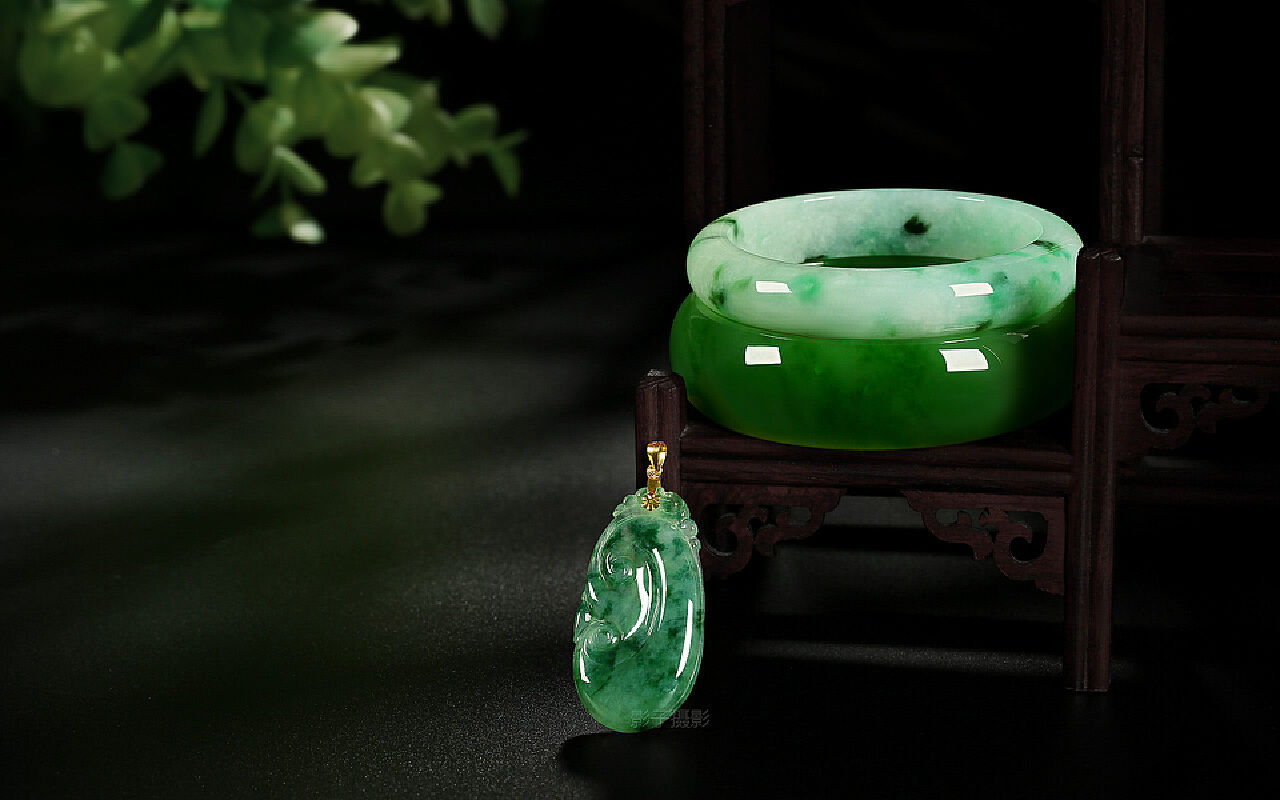
\includegraphics[width=0.8\textwidth]{fig008.jpg}  % Replace "example-image" with the file name of your image
	\caption{Jade Appreciation}
	\label{fig:008}
\end{figure}

\subsection*{Learning from the Best: Guest Experts in the Field}

As if Professor Zhou’s lectures weren’t enough, he regularly invites guest speakers—true masters of jade craftsmanship and appraisal. These experts come from all corners of the jade industry, from artists who carve exquisite sculptures to dealers who trade in some of the finest jade pieces in the market.

Listening to these masters is nothing short of fascinating. They have the ability to look at a piece of jade and immediately evaluate its origin, quality, and value. What’s more, their insights into the contemporary jade market add a modern layer to our traditional studies. I particularly enjoyed a recent guest lecture where the expert discussed how the demand for jade has shifted in recent years, influenced by both cultural trends and global trade.

Through these interactions, I’ve gained a deeper understanding of the jade industry, which, like any art form, balances tradition with innovation. It’s not just about the stone itself, but also the craftsmanship, history, and market dynamics that shape how jade is valued and appreciated.

\subsection*{A Visit to the Jade Museum: Learning Beyond the Classroom}

One of the highlights of the course has been the opportunity to visit a \textbf{jade museum}. This field trip gave us a chance to see some of the finest jade artifacts up close—pieces that I’d only ever seen in books or online. The museum was home to an extraordinary collection, spanning thousands of years of Chinese history.

What struck me most during the visit was the sheer diversity of jade objects: from small, intricately carved pendants to massive, ornate sculptures. The museum also featured contemporary jade pieces, showing how this ancient art form is still very much alive today. I spent hours wandering through the exhibits, marveling at the skill and artistry that goes into each piece.

The visit wasn’t just about looking at beautiful objects; it also helped reinforce many of the concepts we’ve been learning in class. I found myself examining pieces with a more critical eye, thinking about the type of jade, the craftsmanship, and even the historical context in which the pieces were created.

\subsection*{A Class Like No Other}

What truly sets this elective apart is how engaging and immersive the learning experience has been. Jade appreciation is more than just a study of stones—it’s a journey through art, history, and culture. Professor Zhou has a unique way of making the material come alive, and the added bonus of jade gifts and expert lectures has made this course truly special.

This elective has also taught me an important lesson: education isn’t just about textbooks and exams. It’s about passion, curiosity, and being open to exploring new worlds—whether that’s through history, art, or even a small piece of jade. As we approach the end of the semester, I can confidently say that this class has not only broadened my understanding of jade but also deepened my appreciation for the rich cultural heritage it represents.

\subsection*{Conclusion}

In conclusion, \textbf{Jade Appreciation} has been the best elective I’ve taken this semester. Between Professor Zhou’s enthusiastic teaching, the surprise jade gifts, guest lectures from top experts, and our trip to the jade museum, this course has been a fascinating journey into the world of jade. It’s rare to find a class that blends history, art, culture, and personal experience so seamlessly, and I’m grateful to have had the opportunity to learn from the best in the field.


\section{Week 15 Diary: Temperature and Human Civilization}

This week, I’ve been reflecting on the fascinating relationship between \textbf{temperature} and the rise and fall of human civilizations. It turns out that climate change isn’t just a modern concern—historically, shifts in weather patterns and temperature have played a pivotal role in shaping human history. I came across some intriguing research by \textbf{Zhu Kezhen}, a renowned Chinese scholar, whose studies revealed that the collapse of several Chinese dynasties was closely linked to significant changes in climate. 

As we delved deeper into this topic, I realized that understanding the connection between temperature and human civilization is not only relevant for understanding the past, but also crucial for predicting future challenges.

\subsection*{The Role of Temperature in Ancient Dynasties}

According to Zhu Kezhen’s research, many ancient Chinese dynasties experienced climate-related difficulties that contributed to their downfall. For instance, the collapse of the \textbf{Shang}, \textbf{Zhou}, and \textbf{Tang} dynasties is believed to have coincided with periods of significant climatic shifts. These shifts often led to either prolonged droughts or unusually cold temperatures, which had a direct impact on agriculture—the backbone of these agrarian societies.

One of the most striking examples is the fall of the \textbf{Ming dynasty}, which, as Zhu noted, was influenced by the \textbf{Little Ice Age}. This period, spanning from the 14th to the 19th century, saw a drop in global temperatures, leading to lower crop yields and widespread famine. For the Ming dynasty, this climatic stress amplified existing political instability, economic struggles, and military pressure. The harsh winters and poor harvests weakened the empire from within, ultimately contributing to its collapse.

\begin{figure}[h!]
	\centering
	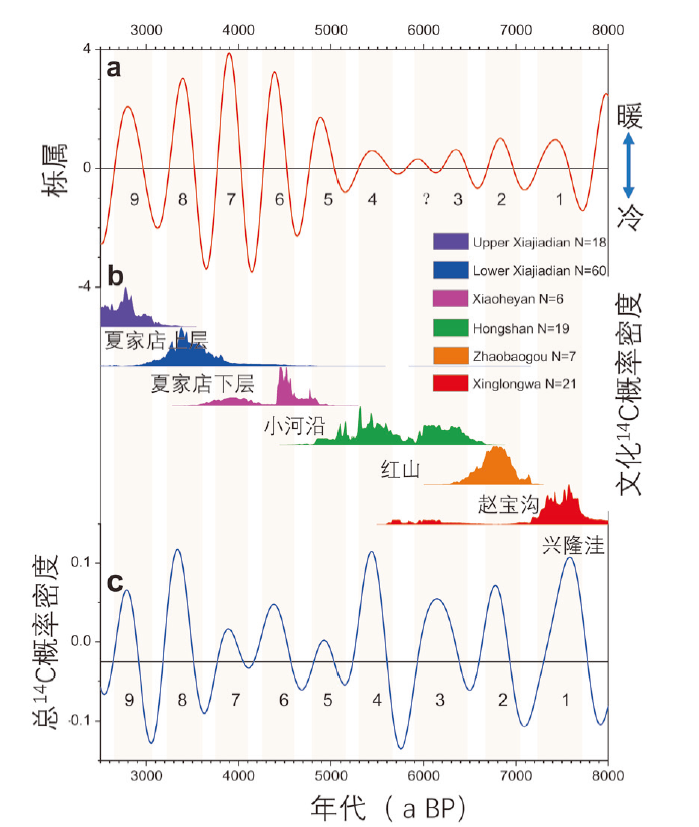
\includegraphics[width=0.8\textwidth]{fig009.png}  % Replace "example-image" with the file name of your image
	\caption{Temperature and Human Civilization}
	\label{fig:009}
\end{figure}

\subsection*{The Little Ice Age and the Ming Dynasty}

The \textbf{Little Ice Age} is one of the most fascinating climatic phenomena in history. During this time, temperatures in the Northern Hemisphere dropped by several degrees. While this might not seem like much, even small changes in average temperature can have devastating effects on food production. In the case of the Ming dynasty, the colder climate led to \textbf{crop failures} and food shortages. Agriculture, which relied heavily on stable weather conditions, was no longer able to support the growing population.

Zhu Kezhen's research highlights how the Ming dynasty struggled to cope with the impacts of the \textbf{Little Ice Age}. The severe winters during the late 16th and early 17th centuries led to poor harvests, which in turn caused widespread famine. This, coupled with political corruption and peasant uprisings, created a perfect storm that the Ming rulers could not weather (pun intended).

What I find most fascinating is how these climatic shifts, which are often seen as background forces in history, can have such direct consequences on human society. It's a reminder that while we often focus on political, social, and economic factors, the environment plays an equally important role in shaping historical outcomes.

\subsection*{A Broader Perspective on Climate and Civilization}

The relationship between temperature and civilization isn’t limited to China. Throughout history, climate changes have had profound effects on societies around the world. The fall of the \textbf{Roman Empire}, for example, has been partially attributed to climatic shifts that affected the Mediterranean region. Similarly, the decline of the \textbf{Maya civilization} in Central America coincided with prolonged periods of drought.

In each of these cases, the changing climate disrupted agricultural production, leading to food shortages, social unrest, and eventually the collapse of political institutions. This pattern underscores the fact that no matter how advanced or powerful a civilization may be, it remains vulnerable to the forces of nature.

Zhu Kezhen’s research has opened my eyes to the complex ways in which climate and human history are intertwined. While political intrigue and military conquest often dominate historical narratives, the influence of temperature and climate should not be overlooked.

\subsection*{Lessons for the Future}

As we face modern-day climate challenges, I can’t help but draw parallels between the past and present. Today, we are grappling with \textbf{global warming}, a different kind of climate shift, but one that is no less dangerous. The historical lessons from the Little Ice Age and the collapse of the Ming dynasty remind us that climate change can—and will—affect human societies in profound ways.

The impacts of climate change are not just an environmental concern; they have far-reaching economic, political, and social implications. The ability of civilizations to adapt to these changes will determine their long-term survival. Just as the Ming dynasty struggled with a cooling climate, modern societies must find ways to mitigate and adapt to the warming world.

\subsection*{Conclusion}

In conclusion, Zhu Kezhen’s research into the relationship between temperature and human civilization has provided me with a deeper understanding of how climate shapes the course of history. From the collapse of the Ming dynasty during the Little Ice Age to the broader impacts of climate on ancient civilizations, it’s clear that temperature plays a critical role in the rise and fall of societies. As we move forward in an era of climate uncertainty, these lessons from the past serve as a reminder that we, too, must adapt to the forces of nature if we hope to secure a sustainable future.


\section{Week 16 Diary: Reflecting on My University Life}

As I near the end of another semester, I can’t help but look back on my journey through university with a mix of nostalgia and exhaustion. It’s been a rollercoaster ride filled with intense competition, endless study sessions, and the ever-present pressure to maintain a high \textbf{GPA}. While the academic experience has certainly been rewarding, I’ve realized that university life is far more demanding than I ever anticipated—far more so than my high school days.

In fact, it sometimes feels like university is not just about learning but about surviving the constant pressures of \textbf{employment}, \textbf{graduate school admissions}, and, of course, keeping that precious GPA above water. The competition is fierce, and there’s little room for relaxation. Every assignment, every quiz, every project seems to carry the weight of the world.

\subsection*{The Datawhale Summer Camp: A Break from GPA Pressure}

One of the few moments in my university life where I truly felt at ease with learning was during the summer break, when I had the opportunity to participate in the \textbf{Datawhale AI Summer Camp}. This experience was nothing short of transformative for me. For the first time in a long while, I found myself learning for the sake of learning, rather than out of fear of lowering my GPA.

The summer camp was focused on \textbf{artificial intelligence}, a field I had always been curious about but never had the time to dive into because of the relentless academic pressure. At the camp, I was able to immerse myself in technical projects, work alongside talented individuals, and receive guidance from AI experts. The best part? There were no grades, no GPA calculations, no looming deadlines—just pure, unadulterated learning.

It was during this camp that I realized how much more enjoyable learning can be when it’s free from the burden of performance metrics. My technical skills improved significantly, and I found joy in tackling challenges, coding solutions, and exploring new concepts without the stress of exams hanging over my head. It was an experience that reignited my passion for learning and reminded me that education is not just about grades—it’s about personal growth.

\subsection*{University Life: Competition, Pressure, and Fatigue}

In contrast, university life has been an entirely different experience. From the moment I stepped onto campus, I could feel the weight of competition. It’s not just about passing; it’s about excelling in every subject, staying ahead of classmates, and positioning oneself for future job opportunities or graduate programs. There’s no room for complacency.

The demands of maintaining a high GPA are relentless. Every quiz, every assignment feels like a test of endurance, and there’s always the fear that one misstep could lower your GPA and jeopardize your future prospects. It’s a system that often leaves little room for creativity or exploration because the focus is on hitting the marks rather than truly engaging with the material.

The constant pressure doesn’t stop at academics, either. The looming specter of \textbf{employment} and \textbf{graduate school admissions} creates an environment where students are perpetually anxious about their future. Networking, internships, job applications—these are all things we are expected to juggle on top of our academic responsibilities. It’s exhausting, and there are times when I wonder if this is how higher education was meant to be.

\begin{figure}[h!]
	\centering
	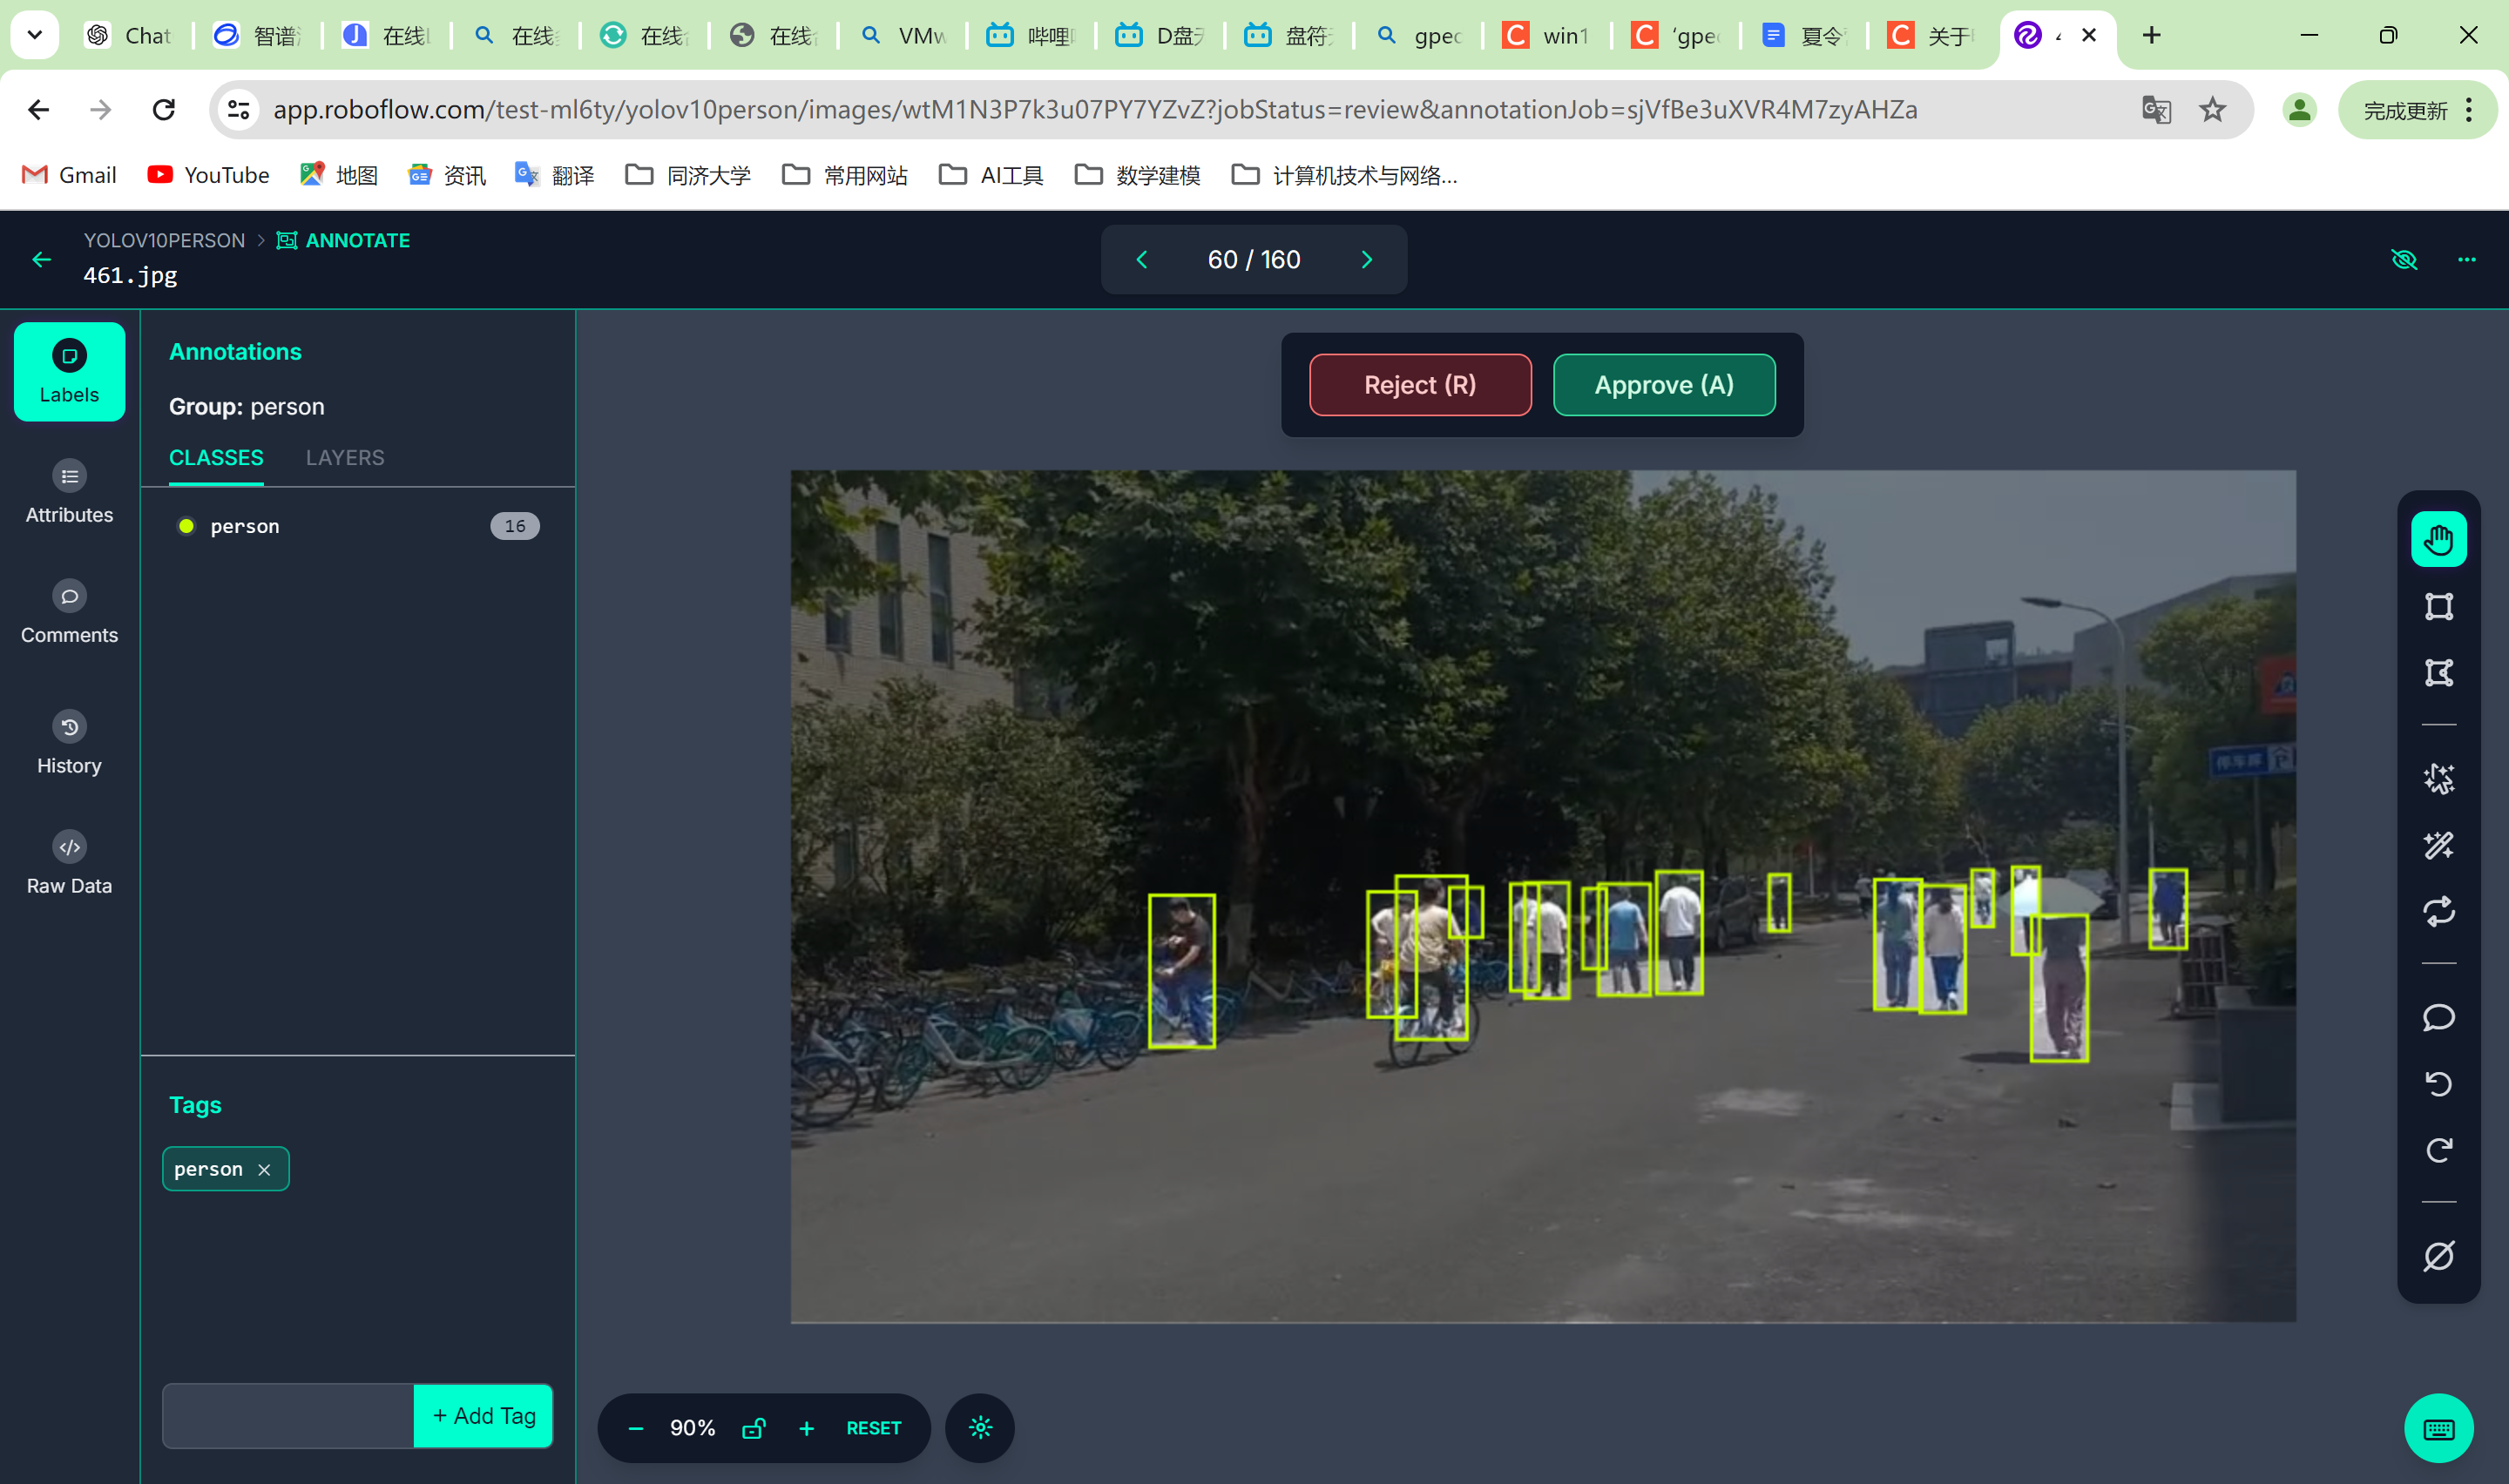
\includegraphics[width=0.8\textwidth]{fig010.png}  % Replace "example-image" with the file name of your image
	\caption{Learning}
	\label{fig:010}
\end{figure}

\subsection*{A Reflection on the Unreasonableness of University Pressure}

As I reflect on these experiences, I can’t help but feel that something is fundamentally wrong with the way university life has become so focused on metrics like GPA, job prospects, and competition. Learning should be about curiosity, exploration, and growth—not about constant stress and burnout.

\begin{figure}[h!]
	\centering
	
\includegraphics[width=0.8\textwidth]{fig011.jpg}  % Replace "example-image" with the file name of your image
	\caption{certificate}
	\label{fig:011}
\end{figure}

The summer camp with \textbf{Datawhale} reminded me of the joy of learning without pressure, and I wish that more of my university experience could be like that. The idea that students are under constant strain just to survive in an overly competitive environment seems, quite frankly, unreasonable. Education should inspire, not exhaust. It should empower, not drain.

\subsection*{Conclusion}

In conclusion, my university journey so far has been a tale of two extremes: the joy of learning without pressure during the \textbf{Datawhale AI Summer Camp} and the exhausting, competition-driven reality of everyday university life. While I’ve learned a lot, I can’t help but feel that the current system places too much emphasis on grades and not enough on the actual experience of learning. As I move forward, I hope to find a balance between pursuing academic success and maintaining my passion for learning—without letting the pressures of competition and GPA weigh me down.

\section{Week 17 Diary: Closing Reflections on the Course}

As this semester draws to a close, I find myself looking back on the journey that has been both challenging and rewarding. This week marks the end of our academic schedule, and with it comes the inevitable countdown to final exams. While it’s tempting to focus solely on the stress of exam preparation, I want to take a moment to reflect on the broader experience of the semester, especially in this \textbf{Academic English Writing} course, which has pushed me to grow as a writer and thinker.

It’s been a semester full of learning, both in and outside the classroom, and as we prepare to wrap things up, I realize just how much I’ve gained—not just in terms of academic knowledge but also in terms of personal development. The process of working through weekly diaries, like this one, has helped me sharpen my ability to express complex ideas clearly and concisely, all while maintaining an academic tone.

\subsection*{The Journey Through the Semester}

Looking back, the semester feels like a marathon. From the early weeks of getting back into the rhythm of academic life to the intense moments of juggling multiple assignments and projects, it’s been a whirlwind. Each week brought its own set of challenges, whether it was grasping difficult concepts in other courses, or refining my ability to write persuasively in this class.

One of the key takeaways from this course has been learning the value of \textbf{structured writing}. Writing weekly diaries has given me the opportunity to organize my thoughts, reflect on my progress, and express my opinions on various topics in a more formal, academic manner. These diaries, while informal in spirit, have nonetheless required a level of discipline that I didn’t anticipate. Crafting coherent narratives, using clear arguments, and maintaining a formal yet engaging tone have all been skills that I’ve honed over the weeks.

\subsection*{Preparing for Final Exams: The Final Stretch}

Of course, while this diary is reflective, the reality of the next couple of weeks cannot be ignored. The looming final exams are at the forefront of my mind. It feels like the culmination of everything we’ve learned this semester, and it’s a bit overwhelming to think about how much material we need to review and master in a short amount of time.

The preparation for final exams is both a mental and physical challenge. There are endless notes to review, formulas to memorize, and essays to prepare for. The pressure is real, but I’m trying to approach it with a calm and strategic mindset. I’ve learned that \textbf{prioritization} is key during exam season—knowing which subjects require more focus and which ones I’m already confident in helps me manage my time effectively.

There’s also the realization that, despite the pressure, exams are just one part of the academic experience. While they’re important, they don’t define everything we’ve learned this semester. The true value lies in the knowledge we’ve gained and the skills we’ve developed, both of which extend far beyond the exam room.

\subsection*{Looking Ahead: The End of One Chapter, the Start of Another}

As this semester ends, I’m filled with a mix of relief and anticipation. On one hand, I’m glad to be nearing the finish line and looking forward to a much-needed break. On the other hand, I’m aware that the end of this semester is just the beginning of a new chapter—next semester brings new courses, new challenges, and new opportunities for growth.

The lessons I’ve learned in this course will undoubtedly carry forward. Whether it’s crafting well-structured essays or learning how to balance formal and conversational tones in writing, these skills will serve me well in future academic endeavors. More importantly, I’ve gained a deeper appreciation for the process of writing itself. Writing is not just about putting words on paper; it’s about communicating ideas effectively and engaging with the reader in a meaningful way.

\subsection*{Conclusion: Farewell to the Semester}

In conclusion, this semester has been a journey of growth, reflection, and preparation for the future. The \textbf{Academic English Writing} course, in particular, has helped me refine my writing skills and taught me the importance of clarity and structure. As we gear up for final exams, I’m trying to maintain a positive mindset, focusing on the long-term value of what I’ve learned rather than getting bogged down by the immediate pressure.

As we say goodbye to this semester, I’m looking forward to what comes next, knowing that the skills and experiences from these past months will continue to shape my academic and personal journey. But first—let’s conquer those finals!


%\section*{Acknowledgements}
%My sincere and hearty thanks and appreciations go firstly to my teacher, Mr. Wei wenhao, whose suggestions and encouragement have given me much insight into these knowledges about Anglo-American society and culture. It has been a great privilege and joy to study under his guidance and supervision. Furthermore, it is my honor to benefit from his personality and diligence, which I will treasure my whole life. My gratitude to him knows no bounds.

%I am also extremely grateful to all my friends and classmates who have kindly provided me assistance and companionship in the course of preparing every presentations and debates.

%Finally, I am really grateful to all those who devote much time to reading this movie review and give me much advice, which will benefit me in my later study.

\end{document}
